%%%%%%%%%%%%%%%%%%%%%%%%%%%%%%%%%%%%%%%%%%%%%%%%%%%%%%%%%%%%%%%%%%%%%%%%
%% Customizações do abnTeX2 (http://abnTeX2.googlecode.com)           %%
%% para a Universidade Estadual do Ceara - UECE                       %%
%%                                                                    %%
%% This work may be distributed and/or modified under the             %% 
%% conditions of the LaTeX Project Public License, either version 1.3 %%
%% of this license or (at your option) any later version.             %%
%% The latest version of this license is in                           %%
%%   http://www.latex-project.org/lppl.txt                            %%
%% and version 1.3 or later is part of all distributions of LaTeX     %%
%% version 2005/12/01 or later.                                       %%
%%                                                                    %%
%% This work has the LPPL maintenance status `maintained'.            %%
%%                                                                    %%
%% The Current Maintainer of this work is Thiago Nascimento           %%
%%                                                                    %%
%% Project available on: https://github.com/thiagodnf/uecetex2        %%
%%                                                                    %%
%% Further information about abnTeX2                                  %%
%% are available on http://abntex2.googlecode.com/                    %%
%%                                                                    %%
%%%%%%%%%%%%%%%%%%%%%%%%%%%%%%%%%%%%%%%%%%%%%%%%%%%%%%%%%%%%%%%%%%%%%%%%

%%%%%%%%%%%%%%%%%%%%%%%%%%%%%%%%%%%%%%%%%%%%%%%%%%%%%%%%%%%%%%%%%%%%%%%%
%% Customizações do abnTeX2 (http://abnTeX2.googlecode.com)           %%
%% para a Universidade Estadual do Ceara - UECE                       %%
%%                                                                    %%
%% This work may be distributed and/or modified under the             %% 
%% conditions of the LaTeX Project Public License, either version 1.3 %%
%% of this license or (at your option) any later version.             %%
%% The latest version of this license is in                           %%
%%   http://www.latex-project.org/lppl.txt                            %%
%% and version 1.3 or later is part of all distributions of LaTeX     %%
%% version 2005/12/01 or later.                                       %%
%%                                                                    %%
%% This work has the LPPL maintenance status `maintained'.            %%
%%                                                                    %%
%% The Current Maintainer of this work is Thiago Nascimento           %%
%%                                                                    %%
%% Project available on: https://github.com/thiagodnf/uecetex2        %%
%%                                                                    %%
%% Further information about abnTeX2                                  %%
%% are available on http://abntex2.googlecode.com/                    %%
%%                                                                    %%
%%%%%%%%%%%%%%%%%%%%%%%%%%%%%%%%%%%%%%%%%%%%%%%%%%%%%%%%%%%%%%%%%%%%%%%%

\documentclass[        
    a4paper,          % Tamanho da folha A4
    12pt,             % Tamanho da fonte 12pt
    chapter=TITLE,    % Todos os capitulos devem ter caixa alta
    section=TITLE,    % Todas as secoes devem ter caixa alta
    oneside,          % Usada para impressao em apenas uma face do papel
    english,          % Hifenizacoes em ingles
    spanish,          % Hifenizacoes em espanhol
    brazil            % Ultimo idioma eh o idioma padrao do documento
]{abntex2}

% Importações de pacotes
\usepackage[utf8]{inputenc}                         % Acentuação direta
\usepackage[T1]{fontenc}                            % Codificação da fonte em 8 bits
\usepackage{graphicx}                               % Inserir figuras
\usepackage{amsfonts, amssymb, amsmath}             % Fonte e símbolos matemáticos
\usepackage{booktabs}                               % Comandos para tabelas
\usepackage{verbatim}                               % Texto é interpretado como escrito no documento
\usepackage{multirow, array}                        % Múltiplas linhas e colunas em tabelas
\usepackage{indentfirst}                            % Endenta o primeiro parágrafo de cada seção.
\usepackage{listings}                               % Utilizar codigo fonte no documento
\usepackage{xcolor}
\usepackage{microtype}                              % Para melhorias de justificação?
\usepackage[portuguese,ruled,lined]{algorithm2e}    % Escrever algoritmos
\usepackage{algorithmic}                            % Criar Algoritmos  
%\usepackage{float}                                  % Utilizado para criação de floats
\usepackage{amsgen}
\usepackage{lipsum}                                 % Usar a simulação de texto Lorem Ipsum
%\usepackage{titlesec}                               % Permite alterar os títulos do documento
\usepackage{tocloft}                                % Permite alterar a formatação do Sumário
\usepackage{etoolbox}                               % Usado para alterar a fonte da Section no Sumário
\usepackage[nogroupskip,nonumberlist,acronym]{glossaries}                % Permite fazer o glossario
\usepackage{caption}                                % Altera o comportamento da tag caption
\usepackage[alf, abnt-emphasize=bf, bibjustif, recuo=0cm, abnt-etal-cite=2, abnt-etal-list=0]{abntex2cite}  % Citações padrão ABNT
%\usepackage[bottom]{footmisc}                      % Mantém as notas de rodapé sempre na mesma posição
%\usepackage{times}                                 % Usa a fonte Times
\usepackage{mathptmx}                               % Usa a fonte Times New Roman										
%\usepackage{lmodern}                               % Usa a fonte Latin Modern
%\usepackage{subfig}                                % Posicionamento de figuras
%\usepackage{scalefnt}                              % Permite redimensionar tamanho da fonte
%\usepackage{color, colortbl}                       % Comandos de cores
%\usepackage{lscape}                                % Permite páginas em modo "paisagem"
%\usepackage{ae, aecompl}                           % Fontes de alta qualidade
%\usepackage{picinpar}                              % Dispor imagens em parágrafos
%\usepackage{latexsym}                              % Símbolos matemáticos
%\usepackage{upgreek}                               % Fonte letras gregas
\usepackage{appendix}                               % Gerar o apendice no final do documento
\usepackage{paracol}                                % Criar paragrafos sem identacao
\usepackage{lib/uecetex2}		                    % Biblioteca com as normas da UECE para trabalhos academicos
\usepackage{pdfpages}                               % Incluir pdf no documento
\usepackage{amsmath}                                % Usar equacoes matematicas
\usepackage[section]{placeins}
\usepackage{xcolor}
\definecolor{verde}{rgb}{0.25,0.5,0.35}
\definecolor{jpurple}{rgb}{0.5,0,0.35}
\definecolor{dkgreen}{rgb}{0,0.4,0}
\definecolor{cinza}{rgb}{0.5,0.5,0.5}
\definecolor{mauve}{rgb}{0.58,0,0.82}


\lstset{
  language=Java,
  %basicstyle=\ttfamily\small, 
  keywordstyle=\color{jpurple}\bfseries,
  stringstyle=\color{blue},
  commentstyle=\color{cinza},
  morecomment=[s][\color{blue}]{/**}{*/},
  extendedchars=true,
  showspaces=false,
  showstringspaces=false,
  numberstyle=\tiny\color{gray},
  numbers=left,
  breaklines=true,
  breakautoindent=true, 
  captionpos=b,
  xleftmargin=0pt,
  basicstyle=\ttfamily\tiny,
  tabsize=4,
  inputencoding=utf8,
  extendedchars=true,
  literate=%
        {é}{{\'{e}}}1
        {è}{{\`{e}}}1
        {ê}{{\^{e}}}1
        {ë}{{\¨{e}}}1
        {É}{{\'{E}}}1
        {Ê}{{\^{E}}}1
        {û}{{\^{u}}}1
        {ù}{{\`{u}}}1
        {â}{{\^{a}}}1
        {à}{{\`{a}}}1
        {á}{{\'{a}}}1
        {ã}{{\~{a}}}1
        {Á}{{\'{A}}}1
        {Â}{{\^{A}}}1
        {Ã}{{\~{A}}}1
        {ç}{{\c{c}}}1
        {Ç}{{\c{C}}}1
        {õ}{{\~{o}}}1
        {ó}{{\'{o}}}1
        {ô}{{\^{o}}}1
        {Õ}{{\~{O}}}1
        {Ó}{{\'{O}}}1
        {Ô}{{\^{O}}}1
        {î}{{\^{i}}}1
        {Î}{{\^{I}}}1
        {í}{{\'{i}}}1
        {Í}{{\~{Í}}}1
}

% Organiza e gera a lista de abreviaturas, simbolos e glossario
\makeglossaries

% Gera o Indice do documento
\makeindex


%%%%%%%%%%%%%%%%%%%%%%%%%%%%%%%%%%%%%%%%%%%%%%%%%%%%%
%%          Configuracoes do ueceTeX2              %%
%%%%%%%%%%%%%%%%%%%%%%%%%%%%%%%%%%%%%%%%%%%%%%%%%%%%%

% Opcoes disponiveis

% \trabalhoacademico{tccgraduacao}
%\trabalhoacademico{tccespecializacao}
%\trabalhoacademico{dissertacao}
%\trabalhoacademico{tese}

% Define se o trabalho eh uma qualificacao
% Coloque 'nao' para versao final do trabalho

\ehqualificacao{nao}

% Remove as bordas vermelhas e verdes do PDF gerado
% Coloque 'sim' pare remover

\removerbordasdohyperlink{sim} 

% Adiciona a cor Azul a todos os hyperlinks

\cordohyperlink{nao}

%%%%%%%%%%%%%%%%%%%%%%%%%%%%%%%%%%%%%%%%%%%%%%%%%%%%%
%%          Informação sobre a IES                 %%
%%%%%%%%%%%%%%%%%%%%%%%%%%%%%%%%%%%%%%%%%%%%%%%%%%%%%

\ies{Universidade Estadual do Ceará}
\iessigla{UECE}
\centro{Centro de Ciências e Tecnologia}

%%%%%%%%%%%%%%%%%%%%%%%%%%%%%%%%%%%%%%%%%%%%%%%%%%%%%
%%        Informação para TCC de Graduacao         %%
%%%%%%%%%%%%%%%%%%%%%%%%%%%%%%%%%%%%%%%%%%%%%%%%%%%%%

\graduacaoem{Ciência da Computação}
\habilitacao{bacharel} % Pode colocar tambem 'licenciada'

%%%%%%%%%%%%%%%%%%%%%%%%%%%%%%%%%%%%%%%%%%%%%%%%%%%%%
%%     Informação para TCC de Especializacao       %%
%%%%%%%%%%%%%%%%%%%%%%%%%%%%%%%%%%%%%%%%%%%%%%%%%%%%%

\especializacaoem{Alfabetização de Crianças}

%%%%%%%%%%%%%%%%%%%%%%%%%%%%%%%%%%%%%%%%%%%%%%%%%%%%%
%%         Informação para Dissertacao             %%
%%%%%%%%%%%%%%%%%%%%%%%%%%%%%%%%%%%%%%%%%%%%%%%%%%%%%

\programamestrado{Programa de Pós-Graduação em Ciência da Computação}
\nomedomestrado{Mestrado Acadêmico em Ciência da Computação}
\mestreem{Ciência da Computação}
\areadeconcentracaomestrado{Ciência da Computação}

%%%%%%%%%%%%%%%%%%%%%%%%%%%%%%%%%%%%%%%%%%%%%%%%%%%%%
%%               Informação para Tese              %%
%%%%%%%%%%%%%%%%%%%%%%%%%%%%%%%%%%%%%%%%%%%%%%%%%%%%%

\programadoutorado{Programa de Pós-Graduação em Saúde Coletiva}
\nomedodoutorado{Doutorado em Saúde Coletiva}
\doutorem{Saúde Coletiva}
\areadeconcentracaodoutorado{Saúde Coletiva}

%%%%%%%%%%%%%%%%%%%%%%%%%%%%%%%%%%%%%%%%%%%%%%
%%  Informação relacionadas ao trabalho     %%
%%%%%%%%%%%%%%%%%%%%%%%%%%%%%%%%%%%%%%%%%%%%%%

\autor{Bruno Bezerra Chaves}
\titulo{Métodos Combinatoriais Para Problemas Em Redes Dinâmicas:
Algoritmos De Caminho Mínimo}
\data{2015}
\local{Fortaleza -- Ceará}

% Exemplo: \dataaprovacao{01 de Janeiro de 2012}
\dataaprovacao{13 de Janeiro de 2015}

%%%%%%%%%%%%%%%%%%%%%%%%%%%%%%%%%%%%%%%%%%%%%
%%     Informação sobre o Orientador       %%
%%%%%%%%%%%%%%%%%%%%%%%%%%%%%%%%%%%%%%%%%%%%%

\orientador{Prof. Dr. Marcos José Negreiros Gomes}
\orientadories{Universidade Estadual do Ceará – UECE}
\orientadorcentro{Centro de Ciências e Tecnologia - CCT}
\orientadorfeminino{nao} % Coloque 'sim' se for do sexo feminino

%%%%%%%%%%%%%%%%%%%%%%%%%%%%%%%%%%%%%%%%%%%%%
%%      Informação sobre o Co-orientador   %%
%%%%%%%%%%%%%%%%%%%%%%%%%%%%%%%%%%%%%%%%%%%%%

% Deixe o nome do coorientador em branco para remover do documento

\coorientador{}
\coorientadories{Universidade Co-orientador - SIGLA}
\coorientadorcentro{Centro do Co-orientador - SIGLA}
\coorientadorfeminino{nao} % Coloque 'sim' se for do sexo feminino

%%%%%%%%%%%%%%%%%%%%%%%%%%%%%%%%%%%%%%%%%%%%%
%%      Informação sobre a banca           %%
%%%%%%%%%%%%%%%%%%%%%%%%%%%%%%%%%%%%%%%%%%%%%

% Atenção! Deixe o nome do membro da banca para remover da folha de aprovacao

% Exemplo de uso:
% \membrodabancadois{Prof. Dr. Fulano de Tal}
% \membrodabancadoisies{Universidade Estadual do Ceará - UECE}

\membrodabancadois{Prof. Dr. Albert Einstein Fernandes Muritiba}
\membrodabancadoiscentro{Centro de Tecnologia - CT}
\membrodabancadoisies{Universidade Federal do Ceará -- UFC}
\membrodabancatres{Anal.\textsuperscript{a} MSc. Anderson Bezerra Calixto}
\membrodabancatrescentro{Centro de Ciências e Tecnologia - CCT}
\membrodabancatresies{Empresa Brasileira de Serviços Hospitalares -- EBSERH}
\membrodabancaquatro{}
\membrodabancaquatrocentro{}
\membrodabancaquatroies{}
\membrodabancacinco{}
\membrodabancacincocentro{}
\membrodabancacincoies{}
\membrodabancaseis{}
\membrodabancaseiscentro{}
\membrodabancaseisies{}

\begin{document}	

	% Elementos pré-textuais
	\imprimircapa
	\imprimirfolhaderosto{}
	\imprimirfichacatalografica{elementos-pre-textuais/ficha-catalografica}
	%\imprimirerrata{elementos-pre-textuais/errata}
	\imprimirfolhadeaprovacao
	%\imprimirdedicatoria{elementos-pre-textuais/dedicatoria}
	\imprimiragradecimentos{elementos-pre-textuais/agradecimentos}
	\imprimirepigrafe{elementos-pre-textuais/epigrafe}
	\imprimirresumo{elementos-pre-textuais/resumo}
	\imprimirabstract{elementos-pre-textuais/abstract}
	\imprimirlistadeilustracoes
	\imprimirlistadetabelas
	%\imprimirlistadequadros
	\imprimirlistadealgoritmos
	\imprimirlistadeabreviaturasesiglas	
	%\imprimirlistadesimbolos{elementos-pre-textuais/lista-de-simbolos}   
	\imprimirsumario
	
	%Elementos textuais
	\textual
	\chapter{Introdução}

O Problema de Caminho Mínimo (PCM) é um dos problemas fundamentais da computação, assim como é um problema
clássico em otimização combinatória.
O PCM é intensamente estudado e utilizado em diversas áreas como Engenharia de Transportes, Pesquisa Operacional, Ciência
da Computação e Inteligência Artificial. Isso acontece porque tem potencial de aplicação em
inúmeros problemas que ocorrem em transportes, logística, redes de computadores de
telecomunicações, etc \cite{peer}.

O roteamento de veículos em um sistema de transporte é atualmente uma das aplicações mais comuns.
Neste contexto, vértices representam cruzamento de ruas, os arcos representam as vias
e os pesos representam medida de custo, tempo ou distância. O caminho mínimo entre dois cruzamentos
é dado pelo conjunto de arcos que resulta no custo mínimo do percurso.
Este custo não necessariamente é a menor distância a percorrer,
o conceito é mais genérico, considerando algum atributo quantificável, como,
por exemplo, distância, tempo, risco, etc \cite{boaventura}, \cite{cormen}, \cite{ziviani}.
Através do crescente desenvolvimento dos computadores pessoais ou portáteis, como sistemas
de navegação de carros e sistemas embarcados GPS, esse tipo de problema de caminho mínimo
tem se tornado cada vez mais usado.

Diante o grande aumento do tráfego de veículos, se torna indispensável o uso de sistemas
de previsão de tráfego, que auxiliam o controle de tráfego de veículos.
Através de análises de dados históricos e de tempo real sobre
os dados lidos de fluxo de veículos, informações futuras geradas através de modelos
estatísticos e computacionais podem prever o comportamento do tráfego em determinadas
vias \cite{leonard}.

\section{Motivação}

Um sistema que selecione a melhor rota para os condutores ajudaria a diminuir o tráfego intenso em determinados locais.
Todas essas informações seriam geradas em tempo real e poderia usar Sistemas Inteligentes de Transporte, definidos 
como sistemas de transporte que usam tecnologias de informação e
de telecomunicações buscando reduzir congestionamentos e filas.
Entre as inúmeras aplicações, incluem-se sistemas de apoio à navegação em tempo real, cuja finalidade é auxiliar
motoristas a encontrar os melhores caminhos ou rotas para atingirem seus locais de destino.

Inúmeras aplicações baseadas em Sistemas de Informação Geográfica, ou SIG’s (GIS - \textit{Geographic Information Systems}),
que permitem o tratamento computacional de dados geográficos ou geo-referenciados,
vêm sendo disponibilizadas na Internet.
São ferramentas em forma de mapa que facilitam o usuário localizar um endereço,
encontrar o menor caminho entre dois lugares, ou até mesmo o caminho mais rápido para chegar ao destino \cite{leonard}.

O uso de sistemas ``on-line'' que sugerem a melhor rota de um ponto de origem a um ponto de destino conhecido,
obtém dados em tempo real, e com isso realizam a previsão de rotas otimizadas, levando em conta o tráfego
dentro das diversas faixas de horário, os usuários, etc.
Os usuários que tiverem acesso ao sistema poderiam saber onde há congestionamentos ou qualquer tipo de obstrução das vias.
Isso acontece porque o sistema recebe informações dos veículos, logo ele é considerado um sistema dinâmico,
pois ele se adapta de acordo com os acontecimentos ao longo do tempo.
Para isso, é necessário um algoritmo de caminho mínimo otimizado que forneça uma resposta para o usuário compatível
com o trajeto que irá realizar.

\section{Objetivos}

\subsection{Objetivo Geral}
Criar uma ferramenta que propõe rotas otimizadas entre dois pontos conhecidos ao longo do tempo
numa rede de topologia dinâmica, utilizando o software Dynagraph \cite{dynagraph}.

\subsection{Objetivos Específicos}
\begin{itemize}
 \item Seguir o modelo computacional Dynagraph \cite{dynagraph} para redes dinâmicas para criacão de um modelo composto
 que aborde redes de topologia estática e dinâmica;
 \item Desenvolver uma ferramenta capaz de sugerir um trajeto com menor tempo
 de percurso entre dois pontos conhecidos, baseada no tempo médio de percurso em trechos
 intermediários, numa rede que pode ser alterada ao longo do tempo.
\end{itemize}

\section{Metodologia de Desenvolvimento}

Para o desenvolvimento dessa solução, os grafos utilizados neste trabalho são hipotéticos,
pois a pesquisa se concentra na modelagem do algoritmo de Dijkstra com Radix Heap aplicado a Grafos Dinâmicos.
O trabalho foi dividido em 3 etapas, que são descritas à seguir:

\begin{itemize}
 \item Analisar modelos de Grafos dinâmicos: determinar dentre os modelos existentes o que melhor
 se adapta ao problema proposto;

 \item Empregar modelos de caminhos mínimos: adaptar a aplicação para sistemas que usam 
 previsão dos tempos de percurso;

 \item Efetuar testes: elaborar relatórios através de testes que possam ser analisados pelo
 software de visualização e edição Dynagraph.
\end{itemize}

\section{Organização do Trabalho}

Este trabalho está organizado em cinco capítulos:
O Capítulo 1 apresenta motivações e metodologia para o desenvolvimento da pesquisa.
O Capítulo 2 apresenta uma revisão bibliográfica sobre redes de Topologia Estática, redes Dinâmicas e
sua geração e manutenção, descrevendo algumas soluções.
O Capítulo 3 apresenta a fundamentação teórica para a compreensão do trabalho desenvolvido, abordando
caminhos em grafos estáticos e dinâmicos, e descrevendo os algoritmos desenvolvidos nesta pesquisa.
O Capítulo 4 apresenta os resultados obtidos pelos testes realizados no Dynagraph.
No Capítulo 5 são apresentadas as conclusões deste trabalho e propostas para trabalhos futuros.

	\chapter{Grafos Estáticos e Dinâmicos} \label{grafoestdin}
Segundo \cite{negreirosbook}, um grafo estático é formado por três conjuntos:\\
- Vértice ou Nodos: representam os pontos (N ou V);\\
- Arestas ou Elos: representam ligações não orientadas entre os Nodos (E);\\
- Arcos: representam ligações orientadas entre os vértices (A).\\
O Grafo pode ser representado da seguinte forma: $G(V, E, A)$.

Grafo orientado ou assimétrico - $G(V, A)$, $E = \emptyset$: uma aresta $(u,v)$ é dita orientada de $u$
para $v$ se o par $(u,v)$ for ordenado, com $u$ precedendo $v$.

Numa abordagem computacional, um programa orientado a objetos pode ser associado a um grafo cujos vértices
representam as classes definidas no programa, e cujas arestas indicam a herança entre as classes.
Existe uma aresta de um vértice $v$ a um vértice $u$ se a classe para $v$ estender a classe de $u$.
Logo o grafo é assimétrico, pois essas arestas são dirigidas ou orientadas porque a relação de herança
só existe em uma direção. Outro exemplo segue na figura \ref{fig:assimetrico}.

\begin{figure}[htbp]
\centering
 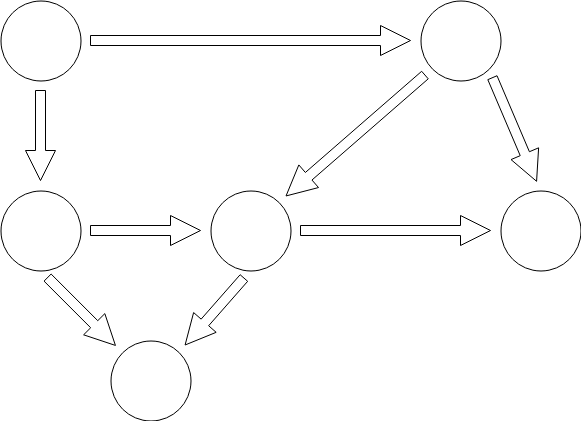
\includegraphics[width=.35\textwidth]{figuras/assimetrico1.png}
\caption{Grafo Orientado ou Assimétrico}
\label{fig:assimetrico}
\end{figure}

Grafo não orientado ou simétrico - $G(V, E)$, $A = \emptyset$: uma aresta $(u,v)$ é dita não-orientada
se o par $(u,v)$ não for ordenado. As aresta não-orientadas são por vezes denotadas como conjunto ${u,v}$,
mas, para simplificar, é utilizado a notação de pares ordenados $(u,v)$, notando que no caso não-orientados
$(u,v)$ é o mesmo que $(v,u)$ \cite{goodrich}, figura \ref{fig:simetrico}.

\begin{figure}[htbp]
\centering
 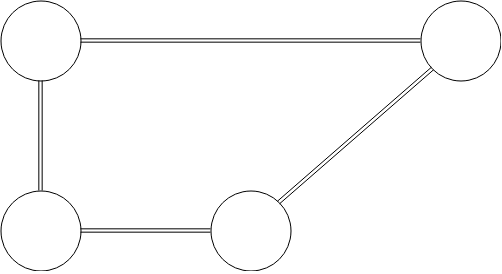
\includegraphics[width=.35\textwidth]{figuras/simetrico1.png}
\caption{Grafo não Orientado ou Simétrico - $G(V,E)$}
\label{fig:simetrico}
\end{figure}
\FloatBarrier

Também é possível visualizar colaborações entre pesquisadores de certa área construindo um grafo cujos vértices são
associados aos pesquisadores e cujas arestas conectam pares de vértices associados aos pesquisadores
que escreveram juntos um artigo ou livro (Figura \ref{fig:goodrich}). Tais arestas são não-orientadas porque
a co-autoria é uma relação simétrica, ou seja, se A é co-autor de B, então necessariamente B é co-autor de A.

\begin{figure}[htbp]
\centering
 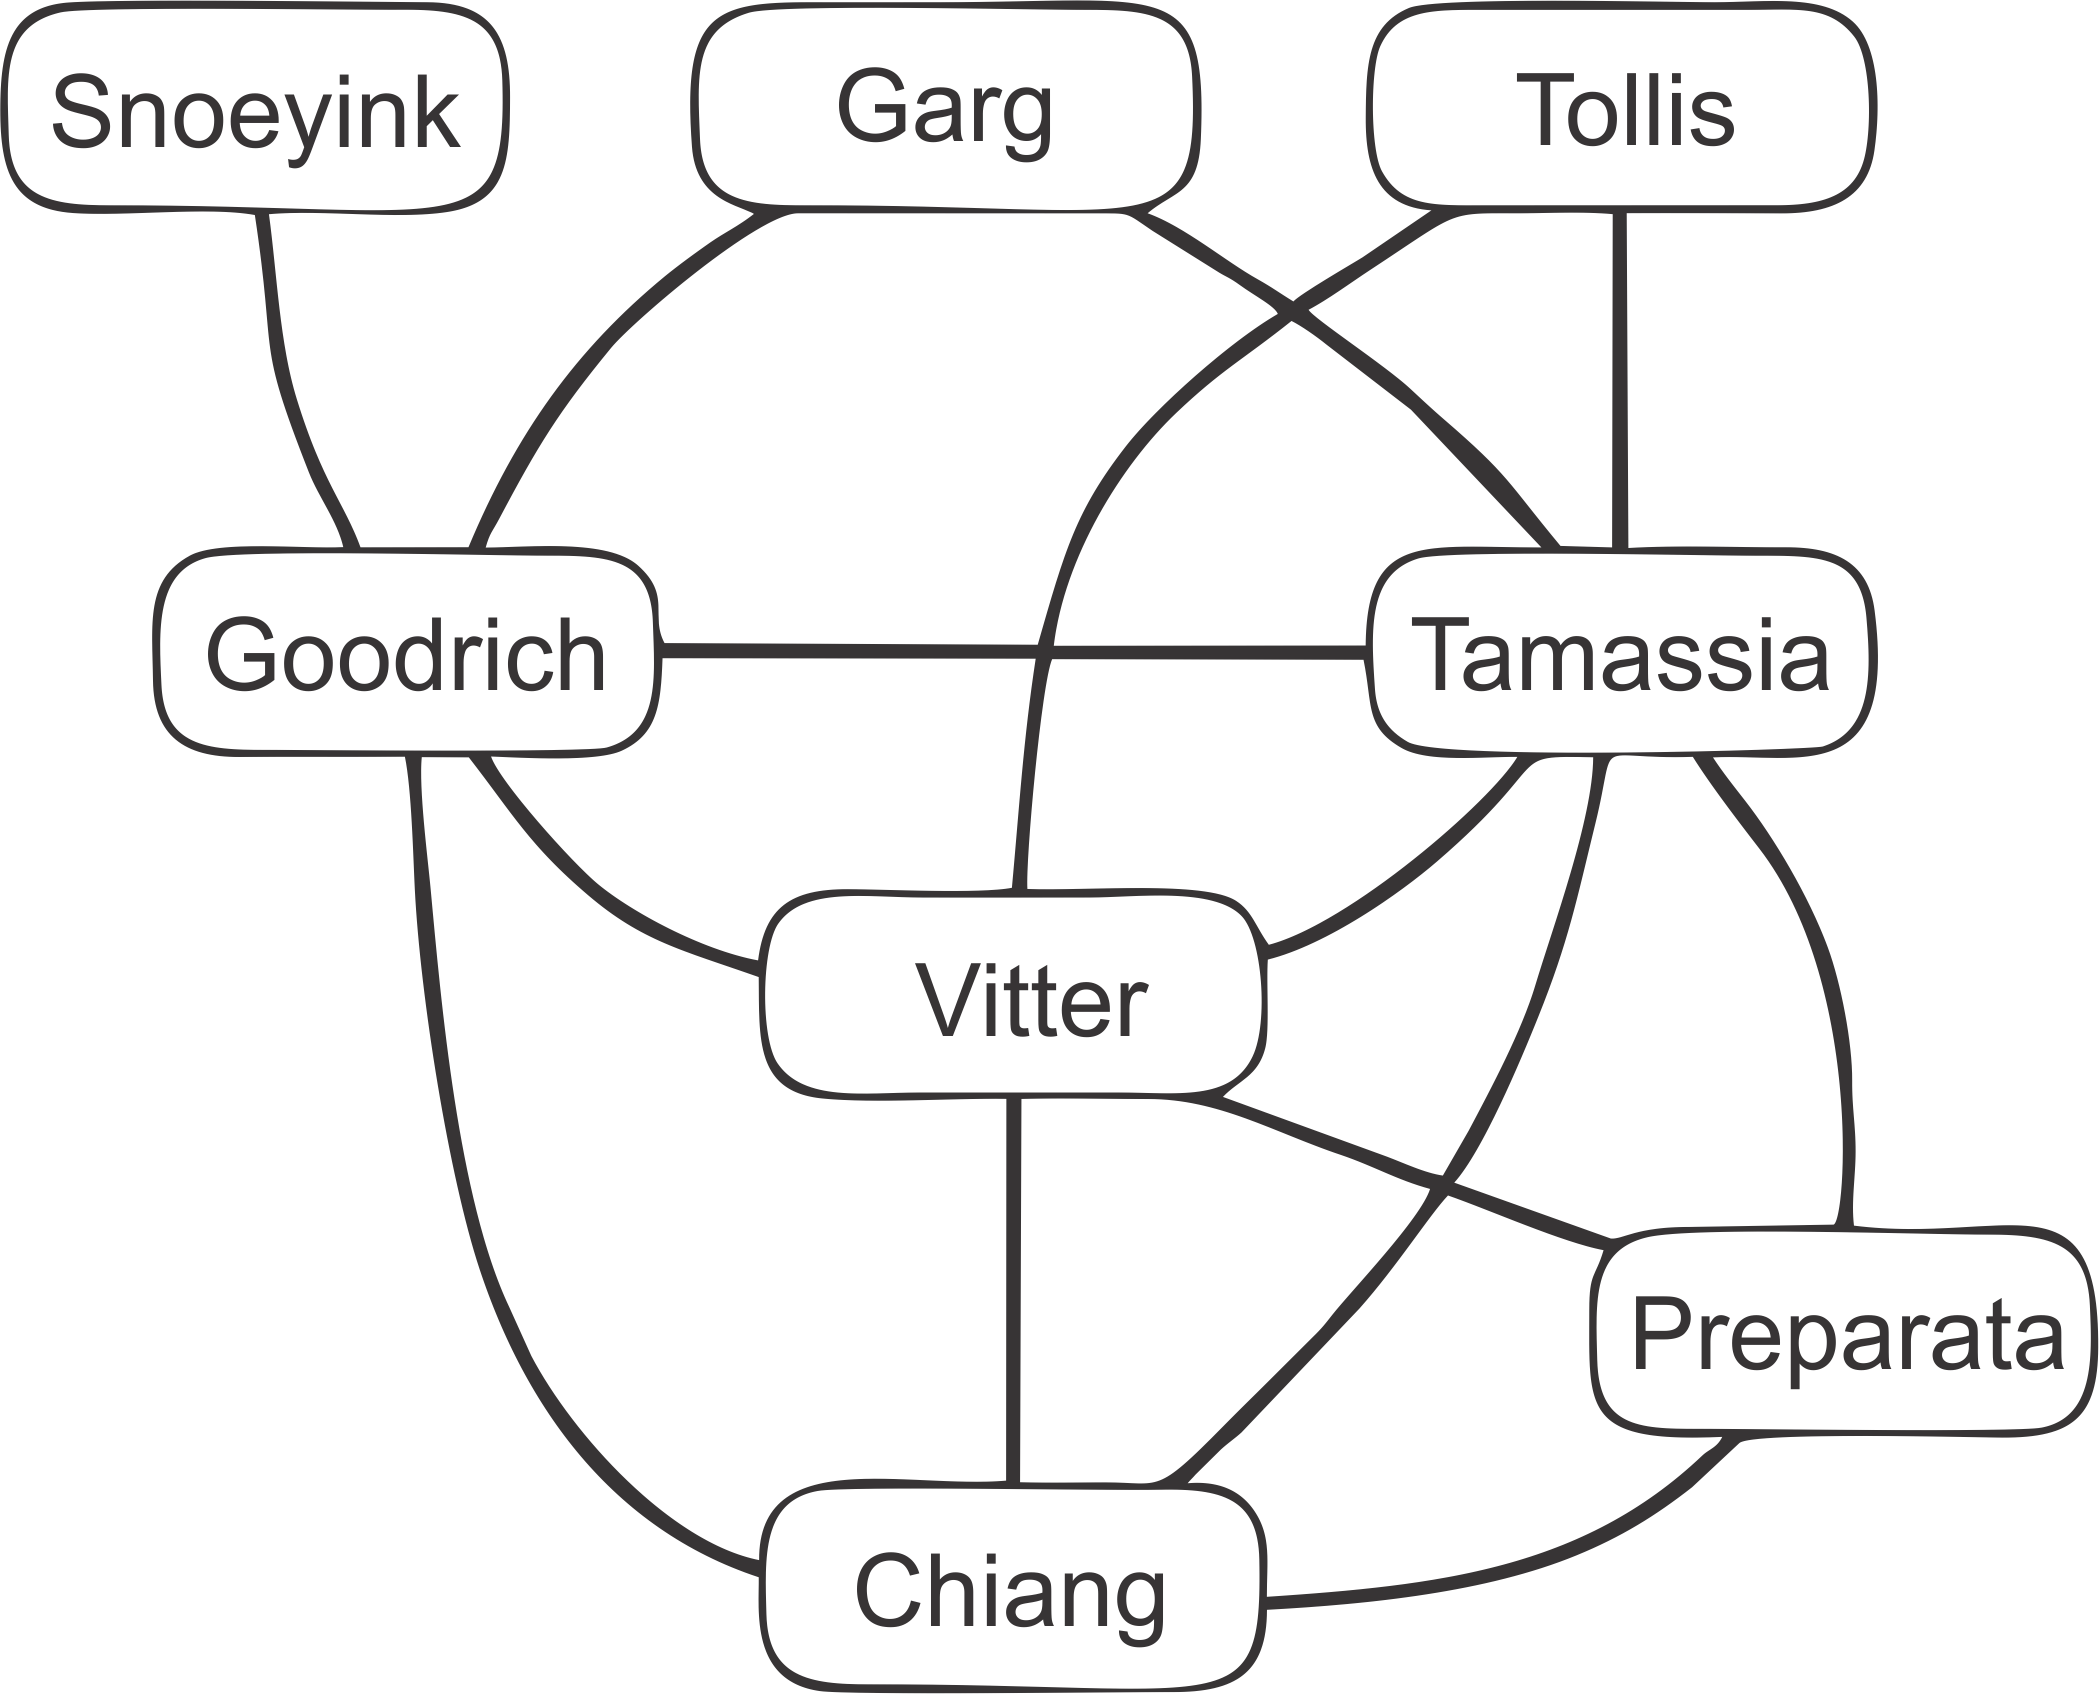
\includegraphics[width=.35\textwidth]{figuras/goodrich.png}
\caption{Grafo de co-autoria de alguns autores}
Fonte: Elaboração própria, baseada em \cite{goodrich}
\label{fig:goodrich}
\end{figure}
\FloatBarrier


Em \cite{goodrich}, se todas as arestas em um grafo forem não-dirigidas,
então diz-se que o grafo é um grafo não-dirigido. De forma similar, um grafo dirigido, ou digrafo, é um grafo em
que todas as arestas são dirigidas. Um grafo que tem arestas dirigidas e não-dirigidas é chamado de grafo misto, 
como mostra a figura \ref{fig:misto}.
Um mapa viário de uma cidade pode ser modelado como um grafo cujos vértices são cruzamentos ou finais de ruas, e cujas arestas
podem ser trechos de ruas sem cruzamentos. Este grafo tem arestas não-dirigidas, representando ruas de dois sentidos,
e arestas dirigidas, correspondendo a trechos de um único sentido. Assim, um grafo que representa as ruas de uma cidade
é um grafo misto.

\begin{figure}[htbp]
\centering
 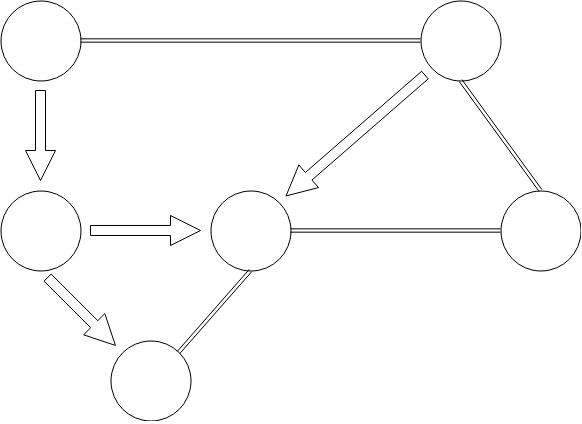
\includegraphics[width=.35\textwidth]{figuras/misto1.png}
\caption{Grafo Misto - $G(V,E,A)$}
\label{fig:misto}
\end{figure}

\section{Rede de Topologia Estática}
Várias estruturas representam esse tipo de rede, como: estrutura matricial,
estrutura de listas encadeadas, estrutura de listas duplamente
encadeadas, dentre outras \cite{negreiros}.
Em  \cite{cormen}, existem duas maneiras para representar um grafo $G = (V,E)$:
como uma coleção de listas de adjacências ou como uma matriz de adjacências. A representação
de lista de adjacências em geral é preferida, porque ela fornece um modo compacto para representar grafos esparsos,
onde para os quais $|E|$ é muito menor que $|V|^2$. Contudo, uma representação de matriz de adjacências pode ser
preferível, quando o grafo é denso, onde $|E|$ está próximo de $|V|^2$, ou quando é preciso ter a possibilidade
de saber com rapidez se existe uma aresta conectando dois vértices dados.

Segundo \cite{goldbarg}, uma matriz $A = |a_{ij}|$ quadrada de ordem $n$ é denominada matriz de adjacência de $G = (V, E)$ quando:\\
\indent $a_{ij}$ = 1, se $\exists(i,j)$ $\in$ $E$\\
\indent $a_{ij}$ = 0 em caso contrário.

As Figuras \ref{fig:matriznaodirecionada} e \ref{fig:matrizdirecionada} apresentam exemplos de matrizes de adjacências para
grafos não orientados e orientados, respectivamente.

\begin{figure}[htbp]
\centering
 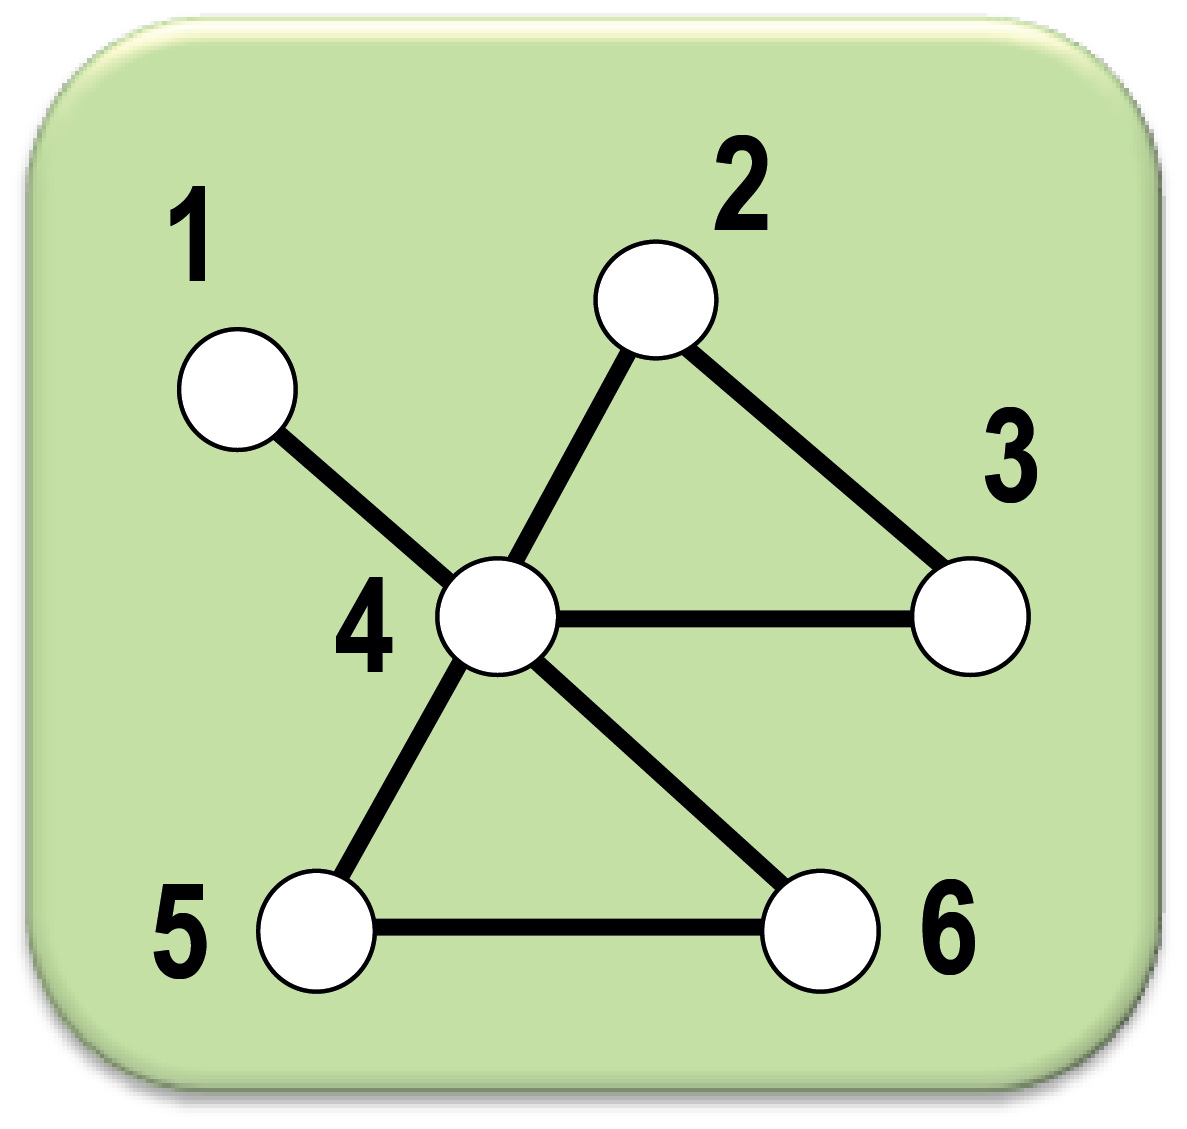
\includegraphics[width=.20\textwidth]{figuras/cal_fig_091a.jpg}
 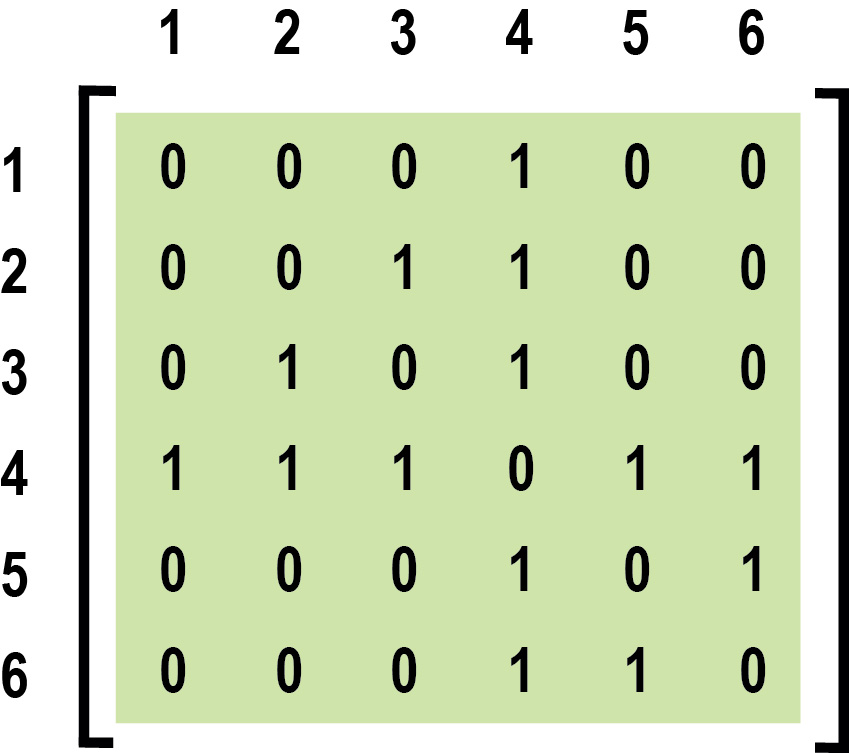
\includegraphics[width=.25\textwidth]{figuras/cal_fig_091b.jpg}
\caption{Matriz de adjacências de grafo não orientado}
Fonte: \cite{goldbarg}
\label{fig:matriznaodirecionada}
\end{figure}

\begin{figure}[htbp]
\centering
 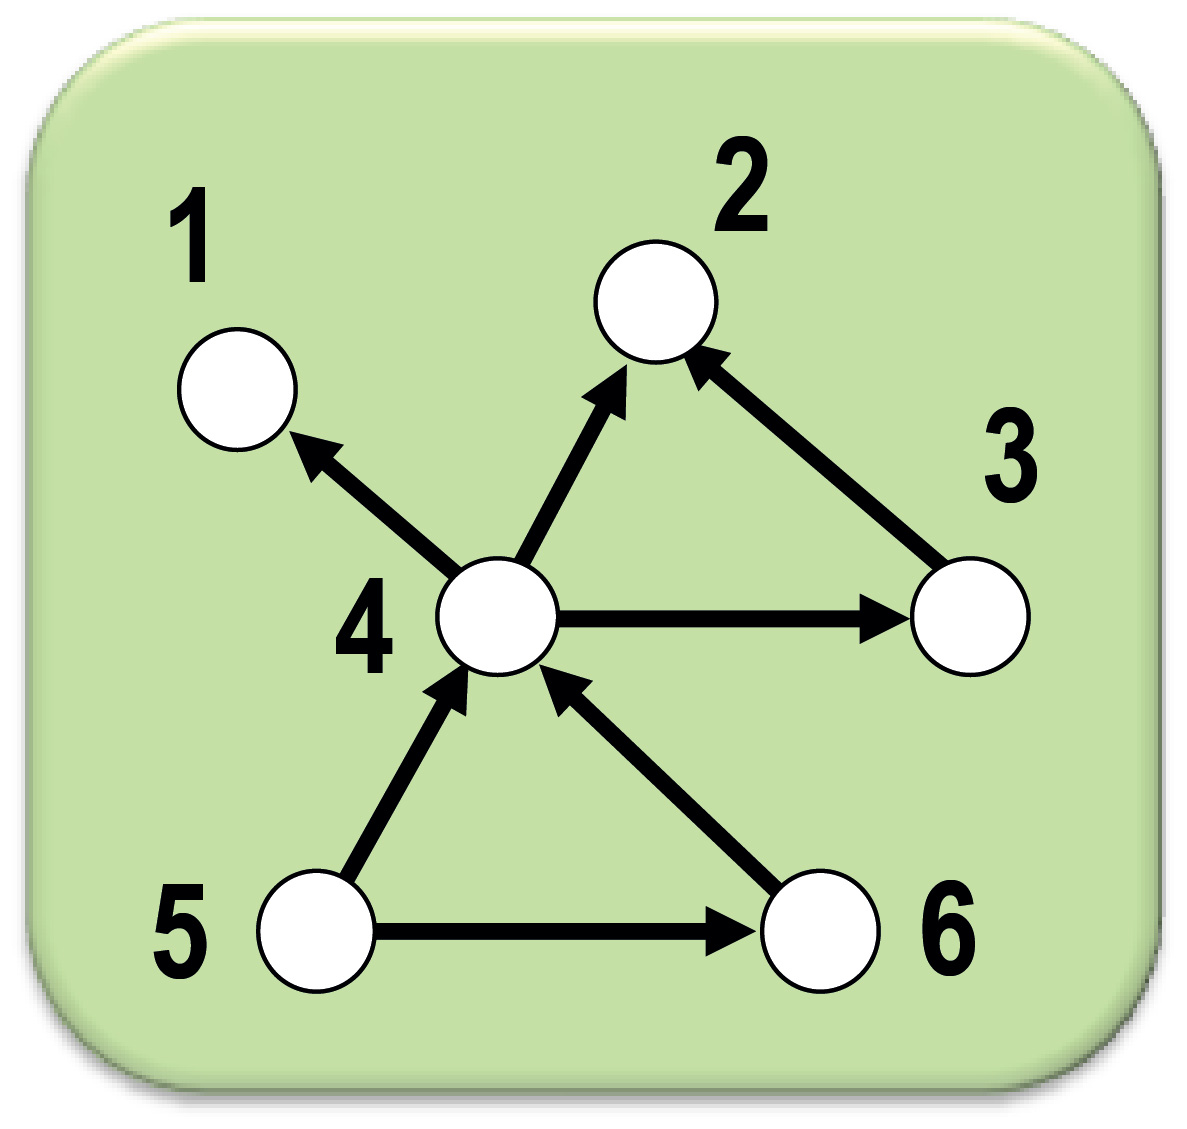
\includegraphics[width=.20\textwidth]{figuras/cal_fig_092a.jpg}
 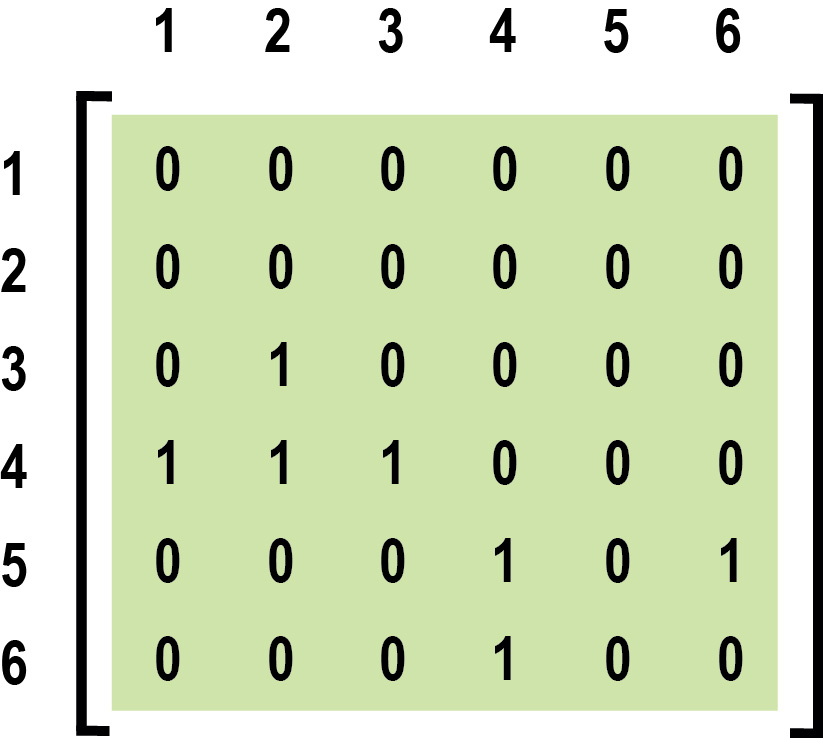
\includegraphics[width=.25\textwidth]{figuras/cal_fig_092b.jpg}
\caption{Matriz de adjacência de grafo orientado}
Fonte: \cite{goldbarg}
\label{fig:matrizdirecionada}
\end{figure}

Em Listas Encadeadas, quando se deseja armazenar um grafo pouco denso, ou seja,
$D_{max} \leqslant$ $\dfrac{|V|}{2}$ é mais vantajoso usar estruturas compactas, assim como as listas
e vetores de listas \cite{negreirosbook}, \cite{cormen}. Neste caso, os vértices estão posicionados no vetor principal,
onde a própria célula do vetor guarda o rótulo do vértice que entrou primeiro e assim sucessivamente, como numa pilha.
As pilhas, que derivam de cada célula do vetor, podem ser construídas levando-se em conta as ligações de arcos/elos ao
elemento vértice da célula que o gera. No índice de cada célula de lista, mantém-se pelo menos uma informação contendo o vértice de ligação,
figura \ref{fig:listaencad}.
\FloatBarrier
\noindent $Type$\\
Lista: $\string^$ Lta;\\
$Lta$ = Record\\
$v$ : word; \{ Arco/elo ligado a VV\_i \}\\
$prx$ : Lista;\\
end;\\
$VV$ = Array[1..n] of Lista;\\

\begin{figure}[htbp]
\centering
 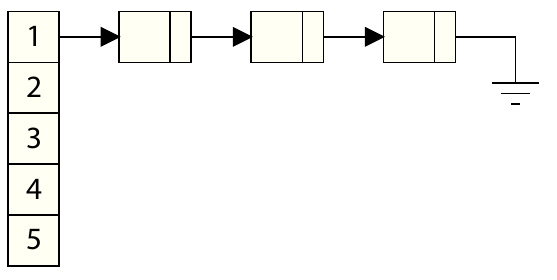
\includegraphics[width=.45\textwidth]{figuras/listaencad.png}
\caption{Representação em Listas Encadeadas de um grafo}
Fonte: \cite{dynagraph} apud \cite{negreirosbook}
\label{fig:listaencad}
\end{figure}

Estruturas de Listas Duplamente Encadeadas são da forma, representada na figura \ref{fig:listdupla}, segundo \cite{negreirosbook}:
\FloatBarrier
\noindent $Type$\\
Lista: $\string^$ Lta;\\
$Lta$ = Record\\
$v$ : word; \{ Arco/elo ligado a VV\_i \}\\
$prx$ : Lista;\\
$ant$ : Lista;\\
end;\\
$VV$ = Array[1..n] of Lista;\\

\begin{figure}[htbp]
\centering
 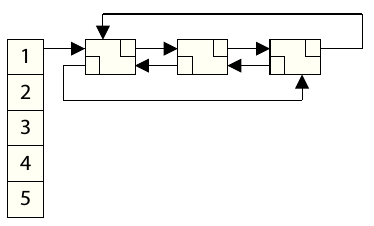
\includegraphics[width=.45\textwidth]{figuras/listdupla.png}
\caption{Representação de um grafo em Listas Duplamente Encadeadas}
Fonte: \cite{dynagraph} apud \cite{negreirosbook}
\label{fig:listdupla}
\end{figure}

\FloatBarrier

\section{Redes Dinâmicas}

Em \cite{harary}, são definidas três tipos de redes: rede de nodos, rede de elos e rede ponderada.
\begin{itemize}
\item Uma rede de nodos (ou grafo de nodos ponderados) é uma tripla $(V, L, f)$, onde $V$ é um conjunto
de vértices, $L$ é um conjunto de ligações $\{u,v\}$, e $f$ é uma função, $f: V \rightarrow N$ onde $N$
é um sistema numérico, atribuição de um valor ou um peso;
\item Uma rede de elos (ou grafo de arestas ponderadas) é uma tripla $(V, L, g)$, definida de forma semelhante a rede de nodos;
\item Uma rede ponderada (ou grafo totalmente ponderado) tem pesos atribuídos a ambos nodos e arestas.
\end{itemize}

Um outro tipo de rede é chamada de rede genérica, que contém atributos e características.

Grafo Dinâmico $G^t(V^t, L^t)$ é todo grafo que modifica seus vértices ($V^t$) e/ou ligações ($L^t$)
ao longo de um período de tempo ($H \in [T_i, T_k]$). Ou seja, as entidades $V$ (um conjunto de nodos),
$L$ (um conjunto de elos), $f$ (mapeamento de vértices para números) e $g$ (mapeamento de arestas para números)
podem se modificar dentro do intervalo H.
Logo, existem cinco tipos básicos de Grafos Dinâmicos:

\begin{itemize}
\item Em um grafo ou digrafo com nós dinâmicos, o conjunto $V$ varia com o tempo. Assim, alguns nós podem
ser adicionados ou removidos. Quando os nós são removidos, as arestas ligadas a eles também são removidas; 
\item Em um grafo ou digrafo com elos ou arcos dinâmicos, o conjunto $L$ varia com o tempo. Assim, as arestas ou arcos podem
ser adicionados ou removidos a partir do grafo ou digrafo;
\item Em um grafo ou digrafo dinâmico de nodos ponderados, a função $f$ varia com o tempo. Assim, os pesos nos nós também variam;
\item Em um grafo ou digrafo dinâmico de elos ou arcos ponderados, a função $g$ varia com o tempo;
\item Em um grafo ou digrafo dinâmico totalmente ponderado (ou grafo com topologia e atributos dinâmicos), ambas as funções $f$ e $g$
podem variar com o tempo.
\end{itemize}

\subsection{Topologia Estática e Atributos Dinâmicos}
Nesta rede, os vértices e as arestas são constantes ao longo do tempo, mas seus atributos podem ser alterados.
O grafo é definido como $G(V^t, L^t)$, onde $V^t$ e $L^t$ são constantes no horizonte $H \in [T_i, T_k]$.
A figura \ref{fig:tead} exemplifica este grafo.

\begin{figure}[htbp]
\centering
 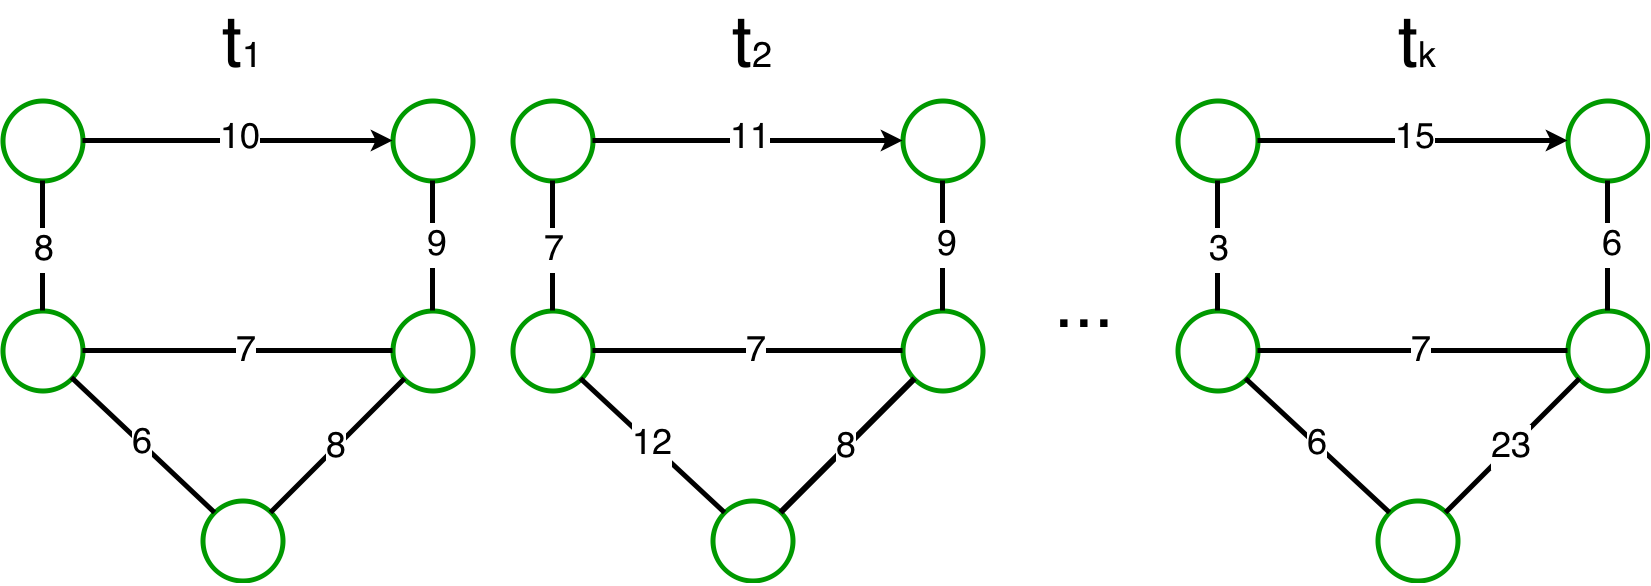
\includegraphics[width=.80\textwidth]{figuras/tead.png}
\caption{Grafo com Topologia Estática e Atributos Dinâmicos}
\label{fig:tead}
\end{figure}

\FloatBarrier

\subsection{Topologia Dinâmica e Atributos Estáticos}
\label{subsec:topdinatribest}
Nesta rede, os vértices e as arestas podem ser removidos, ao longo do tempo, adicionados e até mesmo
modificados para outra posição, mas suas características como espessura, cor e tamanho são fixas.
O grafo é definido como $G(V^t, L^t)$, onde $V^t$ e $L^t$ mudam no horizonte $H \in [T_i, T_k]$,
porém os atributos sempre serão os mesmos. A figura \ref{fig:tdae} mostra um exemplo desse grafo.

\begin{figure}[htbp]
\centering
 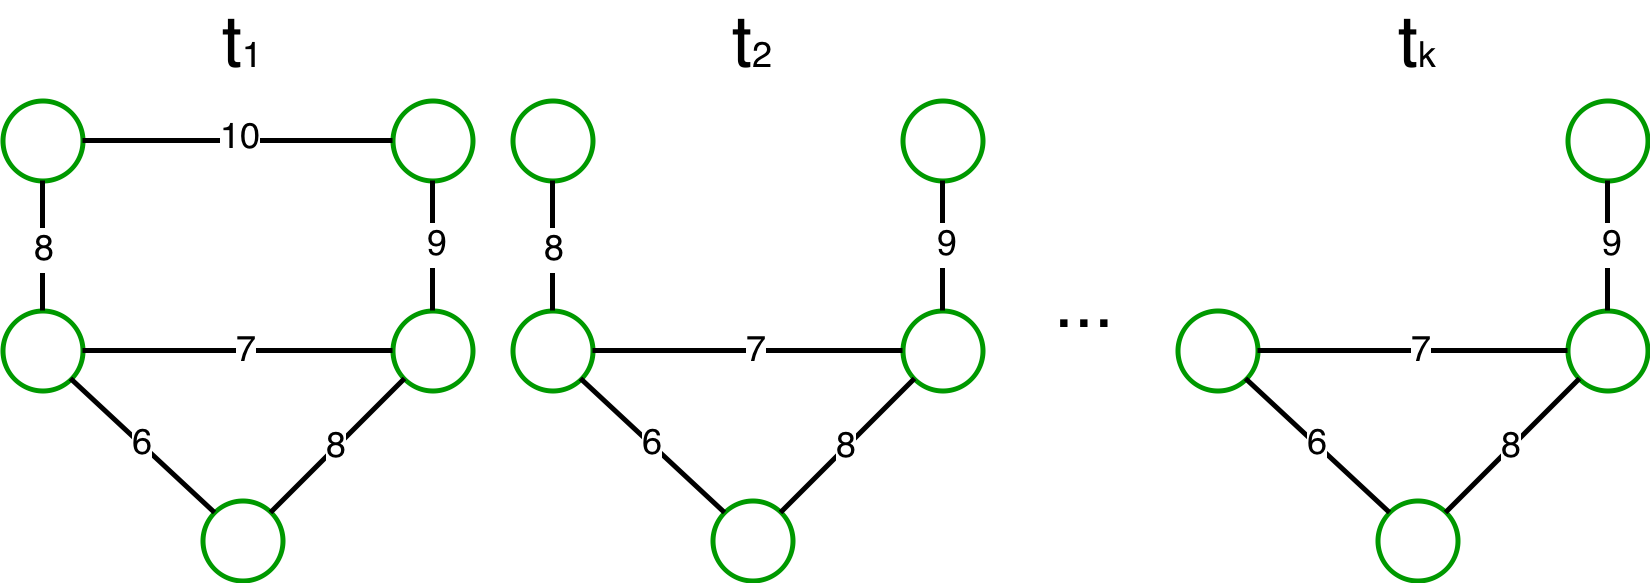
\includegraphics[width=.80\textwidth]{figuras/tdae.png}
\caption{Grafo com Topologia Dinâmica e Atributos Estáticos}
\label{fig:tdae}
\end{figure}

\FloatBarrier

\subsection{Topologia e Atributos Dinâmicos}
\label{subsec:topdinatridin}
Nesta rede os atributos podem ser alterados ao longo do tempo, e o grafo é definido como $G(V^t, L^t)$,
onde $V^t$ e $L^t$ mudam no horizonte $H \in [T_i, T_k]$, como visto na figura \ref{fig:tdad}.
Estas redes são mais complexas \cite{dynagraph}, pois lidam com grande volume de dados comparadas às redes anteriormente descritas.

\begin{figure}[htbp]
\centering
 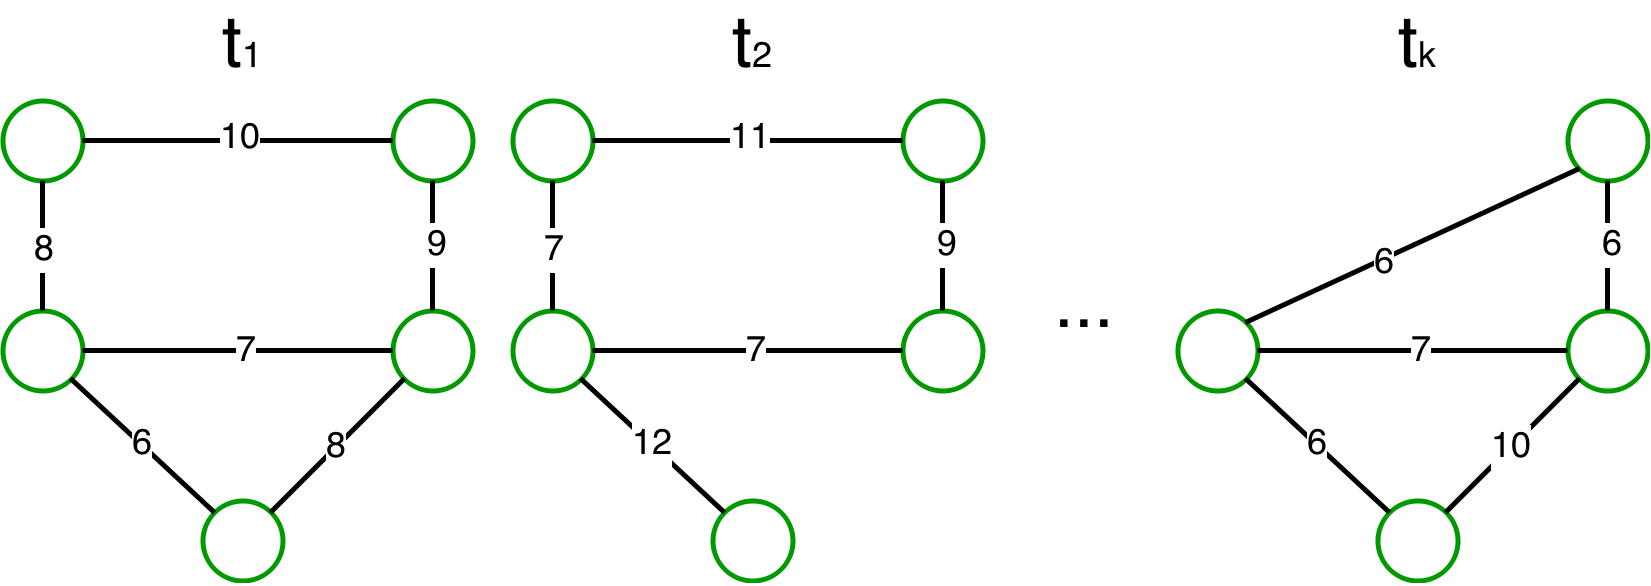
\includegraphics[width=.80\textwidth]{figuras/tdad.png}
\caption{Grafo com Topologia e Atributos Dinâmicos}
\label{fig:tdad}
\end{figure}



\section{Geração e manutenção de Redes Dinâmicas}
Os seguintes trabalhos abordam grafos dinâmicos e são utilizados como base deste trabalho:
\begin{itemize}
\item Modelo de Kim e Anderson, \cite{kim};
\item Gephi, \cite{gephi};
\item Dynagraph, \cite{dynagraph}.
\end{itemize}


\subsection{O modelo de Kim e Anderson}
A ideia central de \cite{kim} é modelar uma rede dinâmica como digrafos orientados
ao tempo \textit{(time-ordered graph)}, que é gerada através da ligação de instantes temporais com arestas
direcionadas que unem cada nó ao seu sucessor no tempo. Com isso, transformar uma rede dinâmica
em um grafo maior, mas facilmente analisável. Isto permite não só a utilização dos algoritmos
desenvolvidos para grafos estáticos, mas também para melhor definir métricas para
grafos dinâmicos.

Segundo \cite{kim} um sistema de grafos dinâmicos é um objeto de representação visual que pode descrever
melhor o comportamento dinâmico de objetos rela\-cio\-nados a eventos dinâmicos e introduzir
novas formas de enxergar ou descrever a evolução de eventos dinâmicos na natureza.

Assumindo que a duração de um período observado é finito, de um tempo inicial $t_{start}$ até o tempo final $t_{end}$, sem perda de
generalidade, é dado $t_{start}$ = $0$ e $t_{end}$ = $T$. Uma rede dinâmica $G^D_{0,T}$ = $(V, E_{0,T})$ consiste
em um conjunto de vértices e arestas temporais existentes no intervalo de tempo $[0,T]$, onde
os vértices $V$ e conjunto de arestas temporais $E_{0,T}$, onde uma aresta $(u,v)_{i,j}$ $\in$ $E_{0,T}$
existe entre vértices $u$ e $v$ em um intervalo de tempo $[i,j]$, tal que $i \leqslant T$ e $j \geqslant 0$ \cite{kim}.

Uma das principais características desse modelo é que o conjunto de vértices $V$ não muda,
enquanto o conjunto de arestas muda ao longo do tempo.

A letra $w$ representa a duração de cada $snapshot$ (ou janela de tempo) e expressa em alguma unidade de tempo (como segundos ou horas).
Uma rede dinâmica pode ser representada como uma série de grafos estáticos $G_1, G_2, ..., G_N$.
A notação $G_t(1 \leqslant t \leqslant n)$ representa o grafo agregado que consiste
de um conjunto de vértices $V$ e um conjunto de arestas $E_t$, onde uma aresta $(u,v)$ $\in$ $E_t$ existe
somente se uma aresta temporal $(u,v)_{i,j}$ $\in$ $E_{0,T}$ existe entre os vértices $v$ e $u$ no intervalo
de tempo $[i,j]$, tal que $i \leqslant wt$ e $j > w(t-1)$. $G_t$ é o t-ésimo $snapshot$ temporal de uma
rede dinâmica $G^D_{0,T}$ durante a t-ésima janela de tempo \cite{kim}.

A tabela \ref{tab:kim} mostra uma relação de arestas e seus intervalos de existência. A figura \ref{fig:grafoKim} mostra os mesmos
dados desta tabela, em uma série de grafos estáticos e representação agredada.

\begin{table}[htbp]
	\centering
	\begin{tabular}{l l l l l l}
	\toprule
	\\Aresta & & & & & Intervalo de tempo\\
	\midrule
	\\(A,C) & & & & & [1,1]\\
	\\(A,D) & & & & & [2,2]\\
	\\(B,D) & & & & & [2,3]\\
	\\(C,D) & & & & & [3,3]\\
	\bottomrule
	\end{tabular}
\caption{Exemplo de contatos (arestas) em uma rede dinâmica}
 \label{tab:kim}
\end{table}

\begin{figure}[htbp]
\centering
 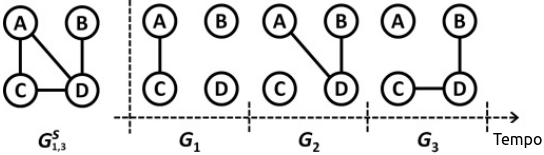
\includegraphics[width=.55\textwidth]{figuras/kim.png}
\caption{Comparação entre a representação de grafos agregados(esquerda) e representação de sequência temporal(direita)}
Fonte: \cite{kim}
\label{fig:grafoKim}
\end{figure}
\FloatBarrier

\subsection{Gephi}
Gephi é um software de código aberto para análise e manipulação de redes.
Ele usa um motor de renderização 3D para exibir grandes redes em tempo real e para acelerar a exploração.
Módulos desenvolvidos podem importar, visualizar, espacializar, filtrar, manipular e exportar todos os tipos de redes \cite{gephi}.

Segundo \cite{dynagraph} o Gephi a princípio, seria um aplicativo para grafos estáticos, porém, posteriormente
foi incorporada uma característica temporal à sua estrutura. Seus dados são baseados em
uma espécie de matriz para vértices e uma outra para arestas. Cada coluna representa uma
informação. Para os vértices, há colunas como identificador, rótulo, posição, tamanho, cor
e intervalo de tempo. Para as arestas, há colunas para o identificador, origem, destino, o
tipo (dirigido ou não), rótulo, peso e cor. No modelo proposto, é possível adicionar novas
colunas para vértices ou arestas, e apenas nestas é possível definir informações que mudam
no tempo.

Como o Gephi não permite que alguns tipos de dados estruturados sejam modificados ao longo do tempo,
os vértices não podem mudar de posição no tempo, tampouco suas características visuais durante a sua existência.
O mesmo acontece com as mudanças de características visuais das arestas, que se mantêm constantes. Apesar
disto, os atributos dos vértices e arestas podem modificar no tempo \cite{dynagraph}. Um adendo importante,
é que vértices e/ou ligações não podem sumir e resurgir no intervalo, limitando a generalidade do Grafo Dinâmico
a ser construído.

As figuras \ref{fig:gephiUm} e \ref{fig:gephiDois} mostram a interface gráfica do Gephi.

\begin{figure}[htbp]
\centering
 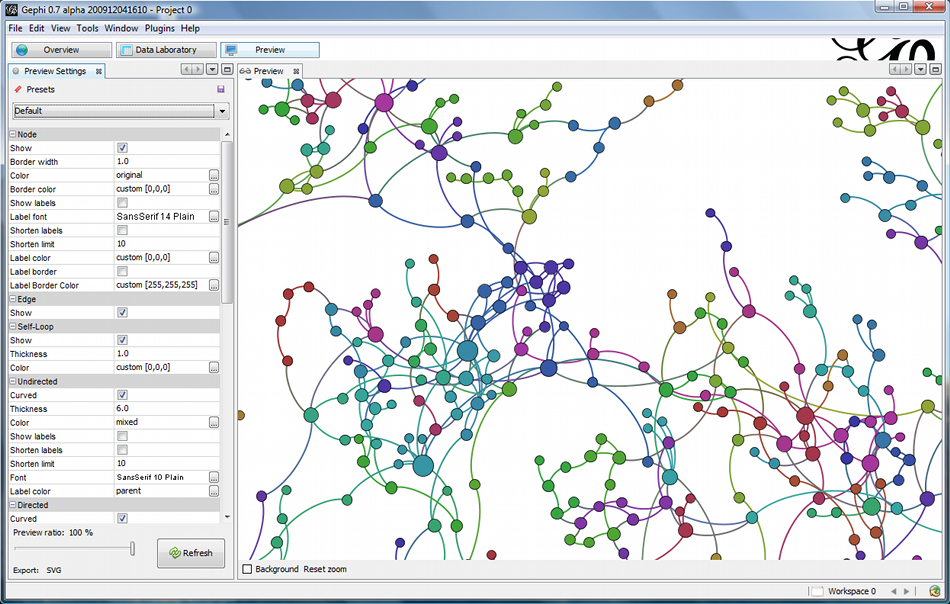
\includegraphics[width=.90\textwidth]{figuras/gephiUm.png}
\caption{Captura de tela do software Gephi}
Fonte: gephi.github.io
\label{fig:gephiUm}
\end{figure}

\begin{figure}[htbp]
\centering
 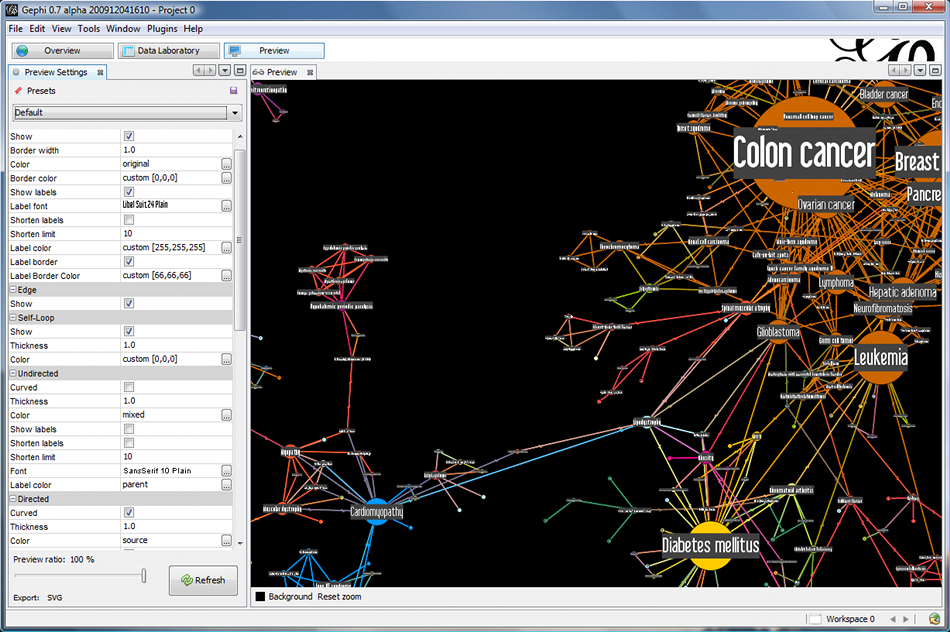
\includegraphics[width=.90\textwidth]{figuras/gephiDois.png}
\caption{Captura de tela do software Gephi}
Fonte: gephi.github.io
\label{fig:gephiDois}
\end{figure}
\FloatBarrier

\pagebreak

\subsection{O modelo Dynagraph}
O modelo Dynagraph \cite{dynagraph} é baseado na primeira proposta em \cite{dynagraph2012}, que por sua vez é baseado no modelo
de \cite{kim}, porém o Dynagraph usa sequências temporais para vértices, arestas, características modificáveis dos vértices e arestas e
o relacionamento entre suas características. Com isso, é formado um grafo com as informações necessárias para qualquer instante no tempo.
O Dynagraph é capaz de visualizar o comportamento do grafo ao longo de um período de tempo, e editá-lo. A ferramenta construída permite
visualizar previsões e processos dinâmicos em vários contextos e realizar simulações preditivas sobre estes eventos \cite{dynagraph}.

Um grafo dinâmico é definido por $G^t$, que ocorre no intervalo $t = [t_s,t_f]$, onde $t_s$ é o tempo inicial e $t_f$ é o tempo final.
$G^t = (V^{t_v}, E^{t_e})$, onde $t_v \subset t$ e $t_e \subset t$, e $V^{t_v}$ e $E^{t_e}$ são funções que geram vértices e arestas
respectivamente, em função do intervalo $t=t_v \cup t_e$.

As estruturas $V^{t_v} = \{O^{t_v}, F^{t_v}\}$ para vértices e $E^{t_e} = \{O^{t_e}, F^{t_e}\}$ para arestas são semelhantes,
onde $O^{t_v} = \{O_{0_v}, O_{1_v},..., O_{i_v}\}$ e $O^{t_e} = \{O_{0_e}, O_{1_e},..., O_{i_e}\}$ são os conjuntos indexados de objetos,
e $F^{t_v} = \{F^{t_v}_{0_v}, F^{t_v}_{1_v},..., F^{t_v}_{w_v}\}$ e $F^{t_e} = \{F^{t_e}_{0_e}, F^{t_e}_{1_e},..., F^{t_e}_{w_e}\}$ são os
conjuntos indexados de características modificáveis de seus respectivos objetos \cite{dynagraph}.

A estrutura de dados usada no Dynagraph segue a Notação de Objeto Javascript (JSON), que é um formato de texto de intercâmbio de dados \cite{douglas}.
A figura \ref{fig:jsondynagraph} mostra como é essa estrutura seguindo três objetos principais: ``metadata'', ``binding'' e ``data''.

Em ``metadata'' são definidos os campos para utilização de qualquer identificador, por exemplo é possível utilizar ``ini'' e ``fim'',
que representam o tempo inicial e final de um elemento, no lugar de ``start'' e ``end'' respectivamente.

Na figura \ref{fig:jsondynagraph}, em ``binding'' são definidas as características dos vértices e arestas.
Seguindo o exemplo da mesma figura, ``vertex'' poderá
ser do tipo ``v1'', ``v2'' e ``v3'', onde cada tipo contém informações da forma do vértice. Essa forma pode ser uma imagem no formato
``png'' ou ``jpg'' ou customizada com as seguintes características:
\begin{itemize}
\item path: círculo ou seta;
\item fillColor: cor do preenchimento;
\item strokeColor: cor da borda;
\item fillOpacity: opacidade;
\item scale: tamanho;
\item strokeWeight: espessura da borda.
\end{itemize}
A aresta, ou ``polyline'', segue uma estrutura semelhante à do ``vertex'', porém com algumas particularidades como repetição de um símbolo
ao longo da aresta, e uma customização no campo ``path'' seguindo a notação
SVG\footnote{\label{note} Scalable Vector Graphics - é uma forma de descrever de forma vetorial desenhos e gráficos bidimensionais}.

Em ``data'' são definidos os elementos do grafo, os tempos de início e fim de cada elemento ou tempo de existência.
No caso dos vértices, a posição de cada elemento pode ser escrita no formato UTM ou latitude e longitude.
O tipo de cada elemento, descrito em ``binding'', e no caso das arestas, são definidos os pontos de origem e destino.

Na figura \ref{fig:jsondynagraph} vemos a estrutura de construção de um grafo dinâmico.
Os campos ``metadata'' e ``binding'' foram omitidos para evidenciar o objeto ``data''.
\FloatBarrier
\lstinputlisting[language=Java]{figuras/new.json}
\begin{figure}[htbp]
  \caption{Estrutura JSON usada pelo Dynagraph}
  \label{fig:jsondynagraph}
\end{figure}

A figura \ref{fig:dynagraph} monstra os dados do código da figura \ref{fig:jsondynagraph} sendo utilizados no software
Dynagraph com variações temporais no grafo e nas características de seus vértices e arestas.

\FloatBarrier
\begin{figure}[htbp]
\centering
 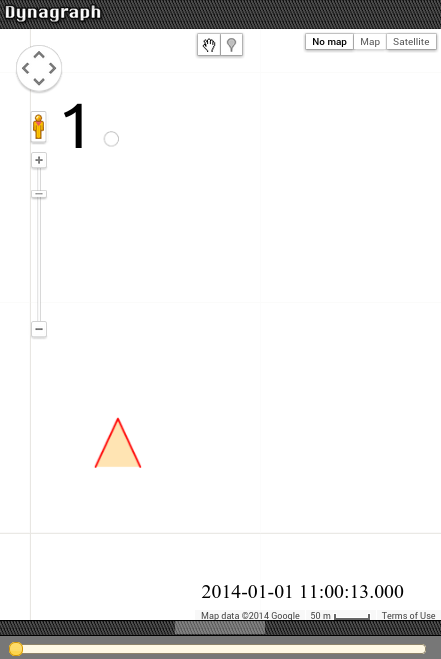
\includegraphics[width=.35\textwidth]{figuras/b1mod.png}
 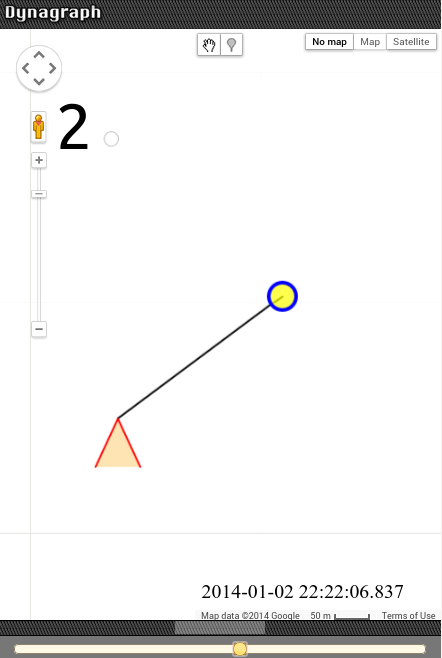
\includegraphics[width=.35\textwidth]{figuras/b2mod.png}
 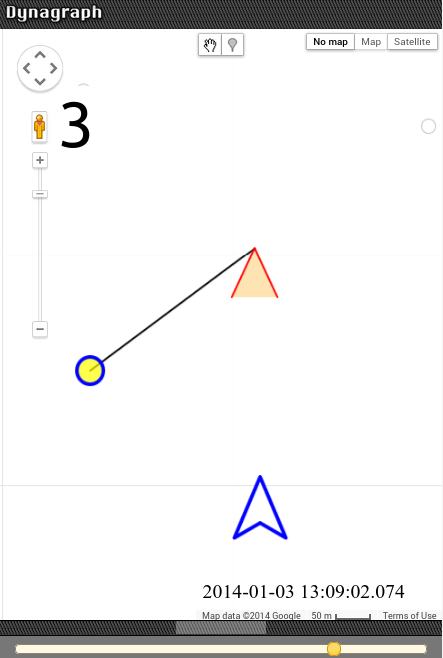
\includegraphics[width=.35\textwidth]{figuras/b3mod.png}
 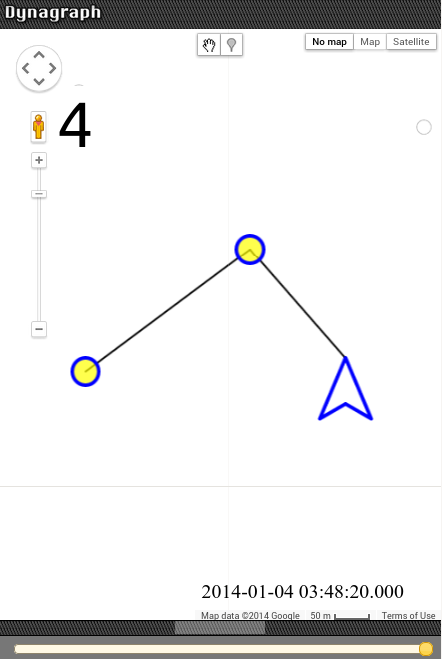
\includegraphics[width=.35\textwidth]{figuras/b4mod.png}
\caption{Capturas de tela do software Dynagraph no modo de edição de um Grafo Dinâmico}
\label{fig:dynagraph}
\end{figure}


	\chapter{Caminhos em Grafos}

\section{Caminhos em Redes Estáticas}
Dentre os diversos problemas que surgem em grafos, este é o mais fundamental de todos e
aquele que ao longo dos anos foi dos mais estudados. Várias técnicas surgiram desde meados
de 1950 com o objetivo de tratar eficientemente o problema de caminhos mínimos em grafos. A
principal delas considera o fato de se promover uma arborescência em um grafo onde à medida
que os vértices explorados são atingidos, tem-se uma proximidade da solução do problema \cite{negreirosbook}.

\subsection{Problema de Caminho Mínimo}
Uma rede de transporte (que pode ser uma malha viária, rodoviária, etc.) pode ser
representada por uma grafo $G = (V, A)$, onde $V$ é o conjunto de nós e A é o conjunto de arcos
os quais interligam estes nós. Considerado o número de nós $|V| = n;$ e o número de arcos $|A| = m;$ para
cada arco $(i, j) \in A$ está associado um custo unitário $c_{ij}$. O caminho entre um
nó origem $(s)$ e um nó destino $(t)$ é definido por uma sequência de
arcos: $(s,i),...(k,l),...(j,t) = \Gamma(s,t)$. O Problema de Caminho Mínimo (PCM) consiste em determinar
um caminho entre $s$ e $t$ tal que a somatória dos custos unitários dos arcos que compõem este caminho seja o mínimo \cite{cunha}.

Dada uma rede $G$ com $m$ nós e $n$ arcos, associando a cada arco $(i,j)$ o custo $c_{ij}$, o Problema
de Caminho Mínimo é encontrar o menor caminho entre o nó 1 e o nó $m$ em $G$ (caminho mínimo de menor valor).
O custo do caminho é dado pela soma dos custos sobre os arcos do caminho encontrado. Uma formatação genérica do problema
de caminho mínimo é dada via grafos, quando deseja-se encontrar o percurso de custo mínimo entre dois vértices $i$ e $j$
de um grafo $G(V,L)$, onde, se $\exists$ $\Gamma (i,j)$, $i$, $j \in V$, então $w_{ij}$ é tomado como o custo mínimo
de um caminho direto entre os vértices $i$ e $j$, e todo $i_1$, ..., $i_k \in V$, distintos de $i$, $j$, são ditos
serem vértices do caminho, onde $i$ precede $i_1$ e assim por diante, nesta ordem \cite{negreirosbook}.

O princípio de qualquer algoritmo de caminho mínimo está associado ao seguinte contexto:
\begin{enumerate}
  \item Seja $G(V,A)$ um grafo dirigido e ponderado, onde $c_{i,j} \geqslant 0, \forall (i,j) \in A$ e $c_{i,j} \in \mathbb{Z}^+$;
  \item G contém um caminho direto entre todo nó $s \in V$ a todo nó $t \in V$;
\end{enumerate}

Propriedade 1: Se o caminho $s=i_1 \rightarrow i_2 \rightarrow \cdots \rightarrow i_h = k$ é o caminho mínimo de s a k ($\Gamma(s,k)$),
então para todo nó $q = 2,3, \cdots, (t-1)$ o subcaminho $s=i_1 \rightarrow i_2 \rightarrow \cdots \rightarrow i_q$ é o menor caminho
do nó fonte ao nó $i_q$.

Propriedade 2: Seja $d$ o vetor que representa as distâncias mais curtas de um vértice s a qualquer vértice t de G. Então o caminho
direto P de um nó fonte a um nó K é um caminho mínimo se e somente se $d(j) = d(i) + c_{ij}$ para todo arco $(i,j) \in P$.

Prova das propriedades pode ser encontrada em \cite{bookahuja}. As propriedades 1 e 2 conduzem ao seguinte teorema representado na
figura \ref{fig:teorema}:

\newtheorem{meuteorema}{Teorema}[chapter]
\begin{meuteorema} \label{teo:Pita} 
Seja $C(\Gamma(s,t))$ o custo do caminho de s a t, então é certo dizer:
$C(\Gamma(s,t)) = C(\Gamma(s,k)) + C(\Gamma(k,t))$ é mínimo $\Longleftrightarrow$ $\Gamma(s,k)$ é mínimo e $\Gamma(k,t)$ é mínimo . 
\end{meuteorema}

\begin{figure}[htbp]
\centering
 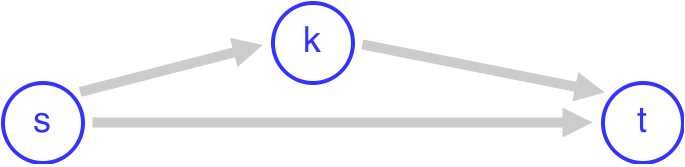
\includegraphics[width=.45\textwidth]{figuras/teorema.png}
\caption{Representação das propriedades do princípio do algoritmo de caminho mínimo}
\label{fig:teorema}
\end{figure}
\FloatBarrier

\subsection{Algoritmo de Dijkstra}
O algoritmo de Dijkstra foi proposto em 1959 e permite determinar a solução ótima através da adição de
vértices à árvore de caminho mínimo pelo processo de relaxamento de uma aresta. Esse processo consiste em verificar
se há a possibilidade de melhorar o caminho obtido até o momento \cite{boaventura}. Este algoritmo considera
basicamente um processo de rotulação de vértices à medida que o menor caminho é encontrado passo a passo,
interativamente, em vértices intermediários. O algoritmo requer que nenhum peso no grafo seja negativo. Abaixo
é apresentado o pseudocódigo do algoritmo de Dijkstra.

\begin{algorithm}[h!]
\Caption{Dijkstra}
  \Inicio{
    inicialize a distância para todos os nós em G = infinito\;
    inicialize o predecessor de todos os nós em G = vazio\;
    \Enqto{H nao estiver vazio}{
      u = o nó com menor rótulo extraído de H\;
      \Para{v=1 até número de adjacentes a u}{
        \Se {rotulo[v] > rotulo[u] + distancia[u, v]}{
          rótulo[v] = rótulo[u] + distância[u, v]\;
          predecessor[v] = u\;
          atualiza a posição de v em H\;
        }
      }
    }
  }
Fonte: \cite{cormen}
\label{newdijkstra}
\end{algorithm}
\FloatBarrier

\subsection{Algoritmo Radix Heap}
O algoritmo Radix Heap é utilizado numa variação do algoritmo de Dijkstra e foi proposto inicialmente por
Ahuja, Mehlhorn, Orlin e Tarjan em \cite{ahuja}.
Ele é considerado ainda no meio científico como um dos algoritmos mais eficientes para resolver o
problema do caminho mínimo.
A implementação do Radix Heap é um híbrido da implementação primitiva $O(n^2)$ e implementação de Dial($O(m + nC))$), que
é uma variação do algoritmo de Dijkstra. 
Estas duas implementações representam dois extremos no que diz respeito à quantidade dos \textit{buckets} utilizados.
A implementação primitiva considera todos os vértices rotulados temporariamente juntos, em um \textit{bucket} grande,
e procura por um vértice com o menor rótulo. Já o algoritmo de Dial usa um grande número de \textit{buckets} e separa os vértices,
armazenando dois vértices quaisquer com rótulos diferentes em diferentes segmentos \cite{bookahuja}.
A implementação Radix Heap melhora esses dois métodos através de uma solução intermediária:
Ele armazena vários, mas não todos os vértices em um mesmo \textit{bucket}. Por exemplo, em vez de armazenar
apenas os vértices com $d[v] = k$ em um \textit{bucket} k, como na implementação do Dial,
pode-se armazenar todos os vértices com $d[v]$ dentro do intervalo [100$k$ para 100$k$ + 99] no \textit{bucket} $k$ \cite{bookahuja}.

Para o \textit{bucket}[k] é definido um intervalo de valores denotado por intervalo(k). O número de inteiros
no intervalo é chamado de largura do intervalo e denotado por largura(k).
No exemplo anterior, o intervalo do \textit{bucket} $k$ é [100$k$, 100$k$ + 99] e sua largura é 100. 

Usar larguras de tamanho $k$ permite reduzir o número de \textit{buckets} necessários por um fator de $k$.
Mas para encontrar o rótulo de menor distância, é preciso procurar todos os elementos no \textit{bucket} não vazio de menor índice.
Para superar isso, o algoritmo radix heap considera usar larguras variáveis e altera os intervalos de forma dinâmica. 
O Radix Heap segue as pro\-prie\-dades:

Propriedade 3: As larguras dos \textit{buckets} são 1, 1, 2, 4, 8, 16, ..., de modo que o número de \textit{buckets} necessários
é somente $O(log_2(NC))$, onde N é o número de vértice e C o custo da maior aresta.

Propriedade 4: Os intervalos dos \textit{buckets} são modificados dinamicamente e são realocados os vértices de menor rótulo temporário
para um único \textit{bucket}, cuja largura é 1.

A Propriedade 3 nos permite manter apenas $O(log_2(NC))$ \textit{buckets} e, assim, supera a desvantagem do algoritmo
de Dial, que usa muitos \textit{buckets}.
A Propriedade 4 nos permite, como no algoritmo Dial, evitar a necessidade de 
pesquisar todo o \textit{bucket} para encontrar um vértice de menor rótulo temporário. Quando implementado deste modo, esta 
versão do algoritmo radix heap tem complexidade $O(m + nlog(nC))$ \cite{bookahuja}.

Para um dado problema de caminho mínimo, o radix heap consiste em formar $1 + [log(NC)]$ \textit{buckets}.
Os \textit{buckets} são numeradas de $0$ até $K = [log(nC)]$.
O algoritmo irá alterar os intervalos dos \textit{buckets} de forma dinâmica, e cada vez que muda os intervalos,
redistribui os vértices nos \textit{buckets}. Inicialmente, os \textit{buckets} têm os seguintes intervalos:\\
intervalo(0) = [0];\\
intervalo(1) = [1];\\
intervalo(2) = [2, 3];\\
intervalo(3) = [4, 7];\\
intervalo(4) = [8, 15];\\
...\\
intervalo(K) = [$2^{K - 1}$, $2^K - 1$].

Esses intervalos mudam à medida que o algoritmo prossegue. No entanto, a largura dos \textit{buckets} nunca aumenta
para além das suas larguras iniciais \cite{bookahuja}.

\subsubsection{Operações sobre o Radix Heap}
Determinar qual intervalo contém um dado valor pode ser feito percorrendo o vetor de \textit{buckets} com complexidade $O(log \hspace*{1mm} nC)$.
Logo, inserir um vértice na estrutura tem complexidade $O(K)$, pois $O(K) = O(log \hspace*{1mm} nC)$

Para descrever a operação de retirar o item da fila de prioridades que contém o menor valor chave considere o seguinte exemplo:
Supondo que o rótulo temporário de um vértice de conteudo(4) é 9, cujo intervalo é [8, 15].
O algoritmo irá examinar cada vértice em conteudo(4) para identificar um vértice com o rótulo de menor distância.
Segundo \cite{bookahuja}, os rótulos de distância que o algoritmo de Dijkstra designa como permanente não são decrescentes,
isso implica que nenhum rótulo temporário de distância jamais voltará
a ser inferior a 9 e, consequentemente, não precisará mais dos \textit{buckets} de 0 a 3.

Em vez de deixar estes \textit{buckets} inativos, o algoritmo redistribui o intervalo [9, 15]
para os \textit{buckets} anteriores, resultando nos intervalos intervalo(0) = [9], intervalo(1) = [10],
intervalo(2) = [11, 12], intervalo(3) = [13,15] e intervalo(4) = $\emptyset$ . Uma vez que o intervalo(4)
está vazio agora, o algoritmo redistribui os vértices que estavam em conteudo(4) para os \textit{buckets} adequados (0, 1, 2, e 3).
Assim, cada um dos vértices no \textit{bucket} 4 move-se para um \textit{bucket} de menor índice e todos vértices com o rótulo de menor distância
são movidos para o \textit{bucket} 0, que tem largura 1 \cite{bookahuja}.

\subsubsection{Funcionamento do Algoritmo de Dijkstra com Radix Heap}
Sempre que o algoritmo encontra vértices com o rótulo de menor distância em um \textit{bucket} com
largura maior que 1, ele verifica todos os vértices no \textit{bucket} para identificar um vértice com rótulo de menor distância.
Em seguida, o algoritmo redistribui o intervalo dos \textit{buckets} e muda cada vértice no \textit{bucket} para o \textit{bucket} de menor índice.
Uma vez que o radix heap contém $k$ \textit{buckets}, um vértice pode mudar na maioria das $k$ vezes, e consequentemente,
o algoritmo irá verificar qualquer vértice na maioria das $k$ vezes. Por isso, o número total de verificações
de vértices é $O(NK)$, o qual não é "muito grande" \cite{bookahuja}.

Para demonstrar o funcionamento do algoritmo de Dijkstra com Radix Heap serão utilizadas figuras do livro \cite{bookahuja}.
O grafo na figura \ref{fig:grafoRadix} exemplifica o radix heap, e o número ao lado de cada arco indica o seu comprimento.
\FloatBarrier
\begin{figure}[htbp]
\centering
 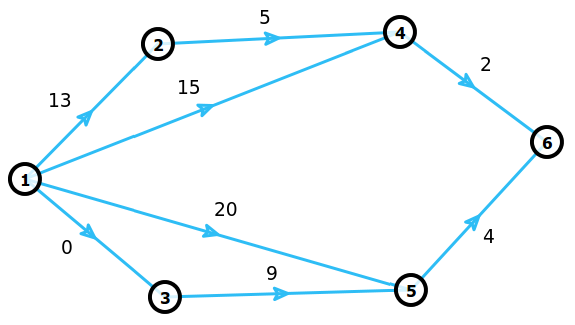
\includegraphics[width=.65\textwidth]{figuras/grafoRadix.png}
\caption{Grafo - Caminho Mínimo}
\label{fig:grafoRadix}
\end{figure}
\FloatBarrier
O vértice origem é $s = 1$. O peso da maior aresta é $C = 20$, logo $K = [log(nC))] = [log(120)] = 7$.
A Tabela \ref{tab:initialradixheap} especifica os rótulos de distância determinada pelo algoritmo de Dijkstra
após análise do vértice 1.
\FloatBarrier
\begin{table}[htbp]
  \centering
  \begin{tabular}{l l l l l l l}
  \toprule
  vértice $i$ & 1 & 2 & 3 & 4 & 5 & 6\\
  \midrule
  rótulo d[$i$] & 0 & 13 & 0 & 15 & 20 & $\infty$ \\
  \bottomrule
  \end{tabular}
  
  \centering
  \begin{tabular}{l l l l l l l l l}
  \toprule
  \\bucket $k$ & 0 & 1 & 2 & 3 & 4 & 5 & 6 & 7\\
  \midrule
  \\intervalo($k$) & [0] & [1] & [2, 3] & [4, 7] & [8, 15] & [16, 31] & [32, 63] & [64, 127]\\
  \\conteudo($k$) & \{3\} & $\emptyset$ & $\emptyset$ & $\emptyset$ & \{2, 4\} & \{5\} & $\emptyset$ & \\
  \bottomrule
  \end{tabular}
\caption{Radix Heap inicial}
 \label{tab:initialradixheap}
\end{table}

Para selecionar o vértice com o rótulo de menor distância, os \textit{buckets} 0, 1, 2, ..., K são percorridos para encontrar o
primeiro \textit{bucket} não vazio. No exemplo, o \textit{bucket} 0 é não vazio. Uma vez que o \textit{bucket} 0 tem largura 1,
cada vértice neste \textit{bucket} tem o mesmo (no mínimo) rótulo de distância. Assim, o algoritmo determina o vértice 3 como permanente,
exclui o vértice 3 do radix heap, e verifica o arco (3, 5) para alterar o rótulo de distância do vértice 5 de 20 para 9.
Em seguida, é verificado se o novo rótulo de distância do vértice 5 está contido no intervalo de seu \textit{bucket} presente,
que é o \textit{bucket} 5. Como o seu rótulo de distância diminuiu, o vértice 5 deve se mover para um \textit{bucket} de menor índice.
Assim, é concluída a análise sequencial dos \textit{bucket} da direita para a esquerda, a partir do \textit{bucket} 5,
para identificar o primeiro \textit{bucket} cujo intervalo contém o número 9, que é o \textit{bucket} 4.
O vértice 5 é movido do \textit{bucket} 5 para \textit{bucket} 4. A tabela \ref{tab:secondradixheap} mostra o novo radix heap.

\begin{table}[htbp]
  \centering
  \begin{tabular}{l l l l l}
  \toprule
  vértice $i$ & 2 & 4 & 5 & 6\\
  \midrule
  rótulo d[$i$] & 13 & 15 & 9 & $\infty$ \\
  \bottomrule
  \end{tabular}
  
  \centering
  \begin{tabular}{l l l l l l l l l}
  \toprule
  \\bucket $k$ & 0 & 1 & 2 & 3 & 4 & 5 & 6 & 7\\
  \midrule
  \\intervalo($k$) & [0] & [1] & [2, 3] & [4, 7] & [8, 15] & [16, 31] & [32, 63] & [64, 127]\\
  \\conteudo($k$) & $\emptyset$ & $\emptyset$ & $\emptyset$ & $\emptyset$ & \{2, 4, 5\} & $\emptyset$ & $\emptyset$ & $\emptyset$\\
  \bottomrule
  \end{tabular}
\caption{Radix Heap - final da iteração 1}
 \label{tab:secondradixheap}
\end{table}
\FloatBarrier
Varrendo os \textit{buckets} sequencialmente, é observado que o \textit{bucket} $k = 4$ é o primeiro \textit{bucket} não vazio.
Uma vez que o intervalo deste \textit{bucket} contém mais de um número inteiro, o primeiro vértice no \textit{bucket} não precisa ter
o rótulo de menor distância. Tem-se que intervalo(4) é [8, 15], mas como seu menor rótulo temporário neste \textit{bucket} é 9,
o novo intervalo a ser redistribuído é o intervalo [9, 15] da seguinte maneira:\\
intervalo(0) = [9],\\
intervalo(1) = [10],\\
intervalo(2) = [11, 12],\\
intervalo(3) = [13, 15],\\
intervalo(4) = $\emptyset$.

Outros intervalos não mudam. Os vértices do \textit{bucket} 4 foram redistribuídos nos \textit{buckets} 0 a 3.
Os \textit{buckets} resultantes têm os seguintes conteúdo:\\
conteúdo(0) = {5},\\
conteúdo(1) = $\emptyset$,\\
conteúdo(2) = $\emptyset$,\\
conteúdo(3) = {2, 4},\\
conteúdo(4) = $\emptyset$.

Esta redistribuição esvazia necessariamente o \textit{bucket} 4 e move o vértice com o rótulo de menor distância para o \textit{bucket} 0.

\subsubsection{Complexidade do Algoritmo de Dijkstra com Radix Heap}
Cada operação de inserção do vértice no \textit{bucket} consome tempo $O(K)$.
Como um vértice só pode ser movido $K$ vezes no máximo, então $O(nK)$ é um limite para o número total de movimentos
de vértices.
O termo $m$ significa o número de distâncias atualizadas, logo o tempo total gasto em atualizar os rótulos temporários
é $O(m + nK)$.
A operação de selecionar um vértice começa verificando os \textit{buckets} da esquerda para a direita para encontrar
o primeiro \textit{bucket} não vazio $k$ no radix heap. Esta operação requer tempo $O(K)$ por iteração e $O(nk)$ no total.
A redistribuição do intervalo segue atribuindo o primeiro inteiro para \textit{bucket} 0, o próximo inteiro para \textit{bucket} 1,
os próximos dois inteiros para \textit{bucket} 2, nos próximos quatro inteiros para \textit{bucket} 3, e assim por diante.
Uma vez que o \textit{bucket} $k$ tem uma largura inferior a $2^{k - 1}$, e uma vez que as larguras dos primeiros $k$ \textit{buckets}
pode ser tão grande como $1, 1, 2, ..., 2^{k - 2}$ até uma largura total de potencial $2k - 1$,
o intervalo útil do \textit{bucket} k sobre os \textit{buckets} $0, 1, ..., k - 1$ é redistribuído.
Esta redistribuição dos intevalos e re-inserções subsequentes de vértices esvazia o \textit{bucket} k e move os vértices com
os rótulos de menor distância para o \textit{bucket} 0 \cite{bookahuja}.
Portanto, como $k = [log(nC)]$, o tempo de execução do algoritmo de Dijkstra com Radix Heap é $O(m + nk) = O(m + n log(nC))$.
Usando a estrutura de dados Fibonacci heap com a implementação do radix heap, é possível reduzir ainda mais a complexidade
para $O(m + n\sqrt{logC})$, o que dá uma execução mais rápida do algoritmo em tempo polinomial para resolver
o problema do caminho mínimo com comprimentos de arcos não negativos \cite{ahuja}.
O algoritmo \ref{codeRadix} apresenta o pseudocódigo do Radix Heap.
% A linha \ref{trechoradix} do algoritmo \ref{codeRadix} 

\begin{algorithm}[h!]
\caption{Radix Heap}
  \Inicio{
    buckets = []\;
    distancias = []\;
    Inicializa o rótulo de distância dos vértices\;
    \Para{i=1 até número de vértices}{
      distancias[i] $\leftarrow$ MAXINT\;
    }
    Inicializa os buckets e seus intervalos\;
    \Para{i=0 até número de buckets}{
      iniBucket $\leftarrow$ $2^{k - 1}$\;
      fimBucket $\leftarrow$ $2^k - 1$\;
    }
    Insere os vértices dentro dos buckets correspondentes\;
    \Enqto{todos os vértices não forem rotulados permanentemente}{
      menorBucket $\leftarrow$ menor bucket não vazio\;
      \Se{o menorBucket tem largura = 1 || número de elementos no menorBucket = 1}{
        verticeSelecionado $\leftarrow$ vértice do menorBucket\;
        \Para{v=0 até número de arcos do verticeSelecionado}{
          Atualiza o rótulo de distância dos vértices \label{trechoradix}\;
          Insere o vértice no bucket que contenha a sua faixa de valores\;
        }
        Remove do heap o verticeSelecionado\;
        Marca o rótulo verticeSelecionado como permanentemente\;
      } \Senao{
        Recalcula o intervalo dos buckets\;
        Redistribui os vertices\;
      }
    }
  }
\label{codeRadix}
\end{algorithm}
\FloatBarrier

\section{Caminhos em Redes Dinâmicas}
\label{sec:pathdyn}
Embora o Problema de Caminho Mínimo seja um dos problemas de otimização combinatória mais bem estudados
na literatura \cite{bookahuja}, Caminhos em Redes Dinâmicas tem recebido muito menos atenção ao longo dos anos.
\cite{giacomo} aborda duas categorias de Problema de Caminho Mínimo em Grafos Dinâmicos. O primeiro é chamado
geralmente na literatura de ``variante dependente do tempo'': nele, o custo de um arco é o tempo de viagem, que é dado
por uma função pré-determinada de tempo, que significa que o custo de um arco $(u, v)$ sobre um caminho
depende do tempo a partir do caminho e do tempo já gasto para alcançar $u$.
O segundo ainda não tem um nome comum na literatura: são grafos onde a função de custo muda ou é atualizada
depois de um certo intervalo de tempo, mas o grafo é estático entre duas alterações da função custo.

\subsection{Algoritmos de Caminho Mínimo Dinâmico}
Esta seção aborda 3 diferentes tipos de grafos, onde se pretende calcular o caminho mais rápido entre pares de vértices
de uma rede dinâmica.
\begin{itemize}
\item $G(V^t, L^t)$ com Topologia Estática e Atributos Dinâmicos;
\item $G(V^t, L^t)$ com Topologia Dinâmica e Atributos Estáticos;
\item $G(V^t, L^t)$ com Topologia Dinâmica e Atributos Dinâmicos.
\end{itemize}

\subsubsection{Topologia Estática e Atributos Dinâmicos}
\label{subsec:limitesuperior}
\cite{leonard} trata o Problema de Caminho Mínimo com previsão de tempo utilizando um vetor de custos e
através da aplicação do algoritmo Dijkstra com Radix Heap modificado. O vetor de custos é composto por dados das passagens 
dos veículos na via como instante da passagem, velocidade, tipo e placa do veículo, que são periodicamente calculados
a cada 10 minutos para cada ligação ou aresta. O algoritmo de Dijkstra é modificado para que o mesmo atualize os custos
de suas arestas à medida que os tempos de percurso se modificam, pois o trânsito dos veículos nas vias descreve um
comportamento dinâmico ao longo do tempo.

Por exemplo, se o tempo parcial até um determinado ponto for de 7 minutos, então
é utilizado para o próximo cálculo o tempo de previsão no intervalo $t + 1$, mas se o tempo parcial for de 15 minutos, logo
o período de previsão é ultrapassado, e com isso utiliza-se $t + 2$ para o cálculo do próximo trajeto. Se o tempo parcial
estiver entre 30 e 40 minutos utiliza-se o intervalo $t + 4$, entre 40 e 50 minutos $t + 5$, e assim por diante.
Essa abordagem é chamada de Algoritmo com Permissão Adiante, pois só altera o intervalo de previsão quando o valor do custo
do vértice for superior a 10.
O algoritmo \ref{codeRadix} representa essa abordagem, e o algoritmo \ref{compermissaoadiante} mostra a modificação
do método na linha \ref{trechoradix} do algoritmo \ref{codeRadix}.

\begin{algorithm}[h!]
\caption{Com Permissão Adiante}
  \Inicio{
    custoAresta $\leftarrow$ horário até o momento\;
    \Se{custoVerticeSelecionado > janelaTemporalAtual}{
      custoAresta $\leftarrow$ tempo de previsão do próximo intervalo\;
    }

    \Se{custoAresta + custoVerticeSelecionado < custoVerticeDestino}{
      custoVerticeDestino $\leftarrow$ custoAresta + custoVerticeSelecionado\;
      predecessor verticeDestino $\leftarrow$ verticeSelecionado\;
    }
  }
\label{compermissaoadiante}
\end{algorithm}
\FloatBarrier

A seguir, é apresentado o funcionamento do algoritmo. O exemplo na figura \ref{fig:leo1} utiliza
6 pontos representados através do grafo G(N=\{P1, P2, P3, P4, P5, P6\}, A).

\begin{figure}[htbp]
\centering
 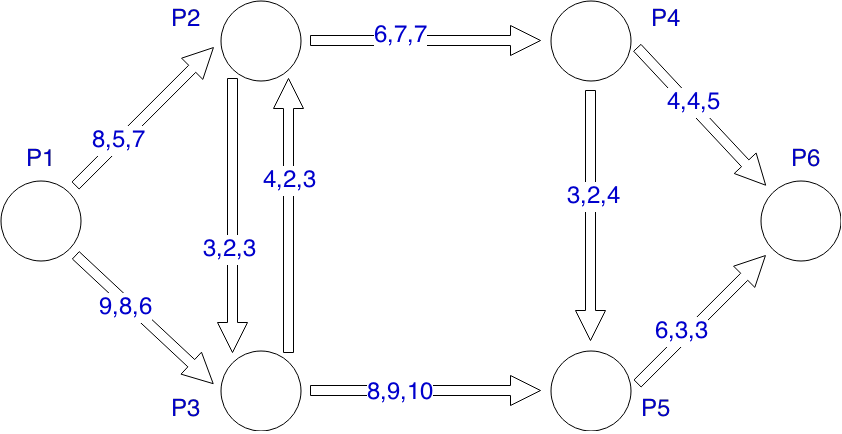
\includegraphics[width=.60\textwidth]{figuras/leo1.png}
\caption{Grafo exemplo para determinação de caminho mínimo}
Fonte: Elaboração própria, baseada em \cite{leonard}
\label{fig:leo1}
\end{figure}

As arestas possuem vários pesos que são os tempos de percursos previstos entre os pontos para os tempos
futuros $t + 1$, $t + 2$ e $t + 3$, como mostra a figura \ref{fig:intervalotemporal}. Esses custos são armazenados
no algoritmo através de um vetor de atributos.
Para determinar o caminho mínimo, utiliza-se um conjunto chamado PERM, que inicialmente contém o vértice fonte P1.
A qualquer momento PERM contém todos os vértices para os quais já foram determinados os menores caminhos usando
apenas vértices em PERM, a partir de P1. Para cada vértice $s$ fora de PERM mantém-se a menor distância dentro do
seu respectivo intervalo de previsão dist[$s$] de P1 a $s$ usando caminhos onde o único vértice que não está em
PERM seja $s$ \cite{leonard}.

\begin{figure}[htbp]
\centering
 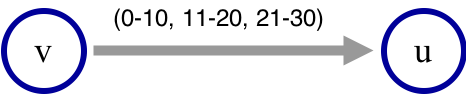
\includegraphics[width=.60\textwidth]{figuras/intervalotemporal.png}
\caption{Representação do intervalo de previsão em uma ligação}
\label{fig:intervalotemporal}
\end{figure}

Outra característica do algoritmo é a necessidade de armazenar o vértice adjacente
a $s$ neste caminho em path[$s$]. Selecionando o vértice com menor distância, entre todos os que ainda não pertencem
a PERM, o adiciona a PERM, chamando-o de $current$, e recalcula-se as distâncias (dist) para todos os vértices
adjacentes a ele que não estejam em PERM, pois pode haver um caminho menor a partir de P1, passando por $current$, 
do que aquele que havia antes de $current$ ser agregado a PERM. É preciso atualizar path[$s$] se houver um caminho
mais curto, e com isso indicar que $current$ é o vértice adjacente a $s$ pelo novo caminho mínimo \cite{leonard}.

Para determinar o caminho mínimo é preciso definir o ponto de origem ou nó raiz. A partir disso, o algoritmo
aplica custo de valor tendendo ao infinito a todos os vértices exceto P1, que possui custo 0. A figura \ref{fig:leo2} exibe
o vértice P1 como ponto de saída. Se o caminho no vértice P1 iniciou no primeiro intervalo (0-10], e vai
até P2, o percurso leva 8 minutos.

\begin{figure}[htbp]
\centering
 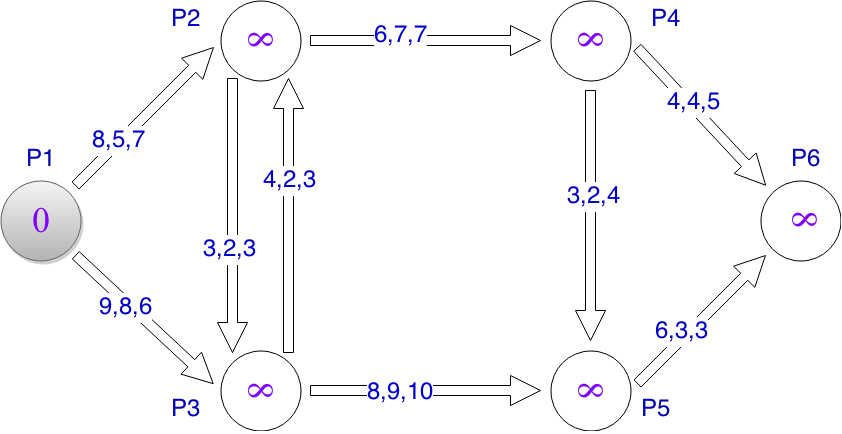
\includegraphics[width=.50\textwidth]{figuras/leo2.png}
\caption{Processo de determinação de caminho mínimo - Parte 1}
\label{fig:leo2}
\end{figure}

\begin{table}[htbp]
  \centering
  \begin{tabular}{l l l l}
  \toprule
  Vértice & PERM & Distância & Predecessor\\
  \midrule
  P1 & Sim & 0 & - \\
  P2 & Não & $\infty$ & - \\
  P3 & Não & $\infty$ & - \\
  P4 & Não & $\infty$ & - \\
  P5 & Não & $\infty$ & - \\
  P6 & Não & $\infty$ & - \\
  \bottomrule
  \end{tabular}
\caption{Processo de determinação de caminho mínimo - Parte 1}
 \label{tab:leotab1}
\end{table}
\FloatBarrier

A partir de P1 consulta-se os vértices adjacentes a ele, que são P2 e P3. Para todos os vértices
adjacentes denonimados $s$, calcula-se o pseudocódigo \ref{compermissaoadiante}.

% \fbox{\begin{minipage}{70ex}
% \vspace*{-1mm} \phantom{} \hspace{3ex} {\bf Se} dist[s] > dist[d]\ + peso(d,s)\\
% \vspace*{-1mm} \phantom{} \hspace{6ex} dist[s] = dist[d]\ + peso(d,s)\\
% \vspace*{-1mm} \phantom{} \hspace{6ex} path[s] = s\\
% \vspace*{-1mm} \phantom{} \hspace{3ex} {\bf Fim Se}\\
% \end{minipage}}
% \begin{figure}[htbp]
% \centering
% \caption{Dijkstra Modificado - Trecho aplicado a vértices adjacentes}
% \label{fig:diMod}
% \end{figure}
% \FloatBarrier

\begin{figure}[htbp]
\centering
 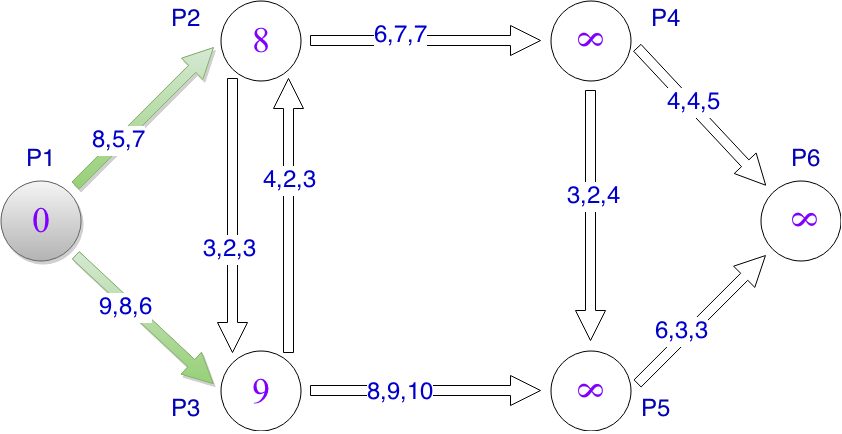
\includegraphics[width=.50\textwidth]{figuras/leo3.png}
\caption{Processo de determinação de caminho mínimo - Parte 2}
\label{fig:leo3}
\end{figure}

\begin{table}[htbp]
  \centering
  \begin{tabular}{l l l l}
  \toprule
  Vértice & PERM & Distância & Predecessor\\
  \midrule
  P1 & Sim & 0 & - \\
  P2 & Não & 8 & P1 \\
  P3 & Não & 9 & P1 \\
  P4 & Não & $\infty$ & - \\
  P5 & Não & $\infty$ & - \\
  P6 & Não & $\infty$ & - \\
  \bottomrule
  \end{tabular}
\caption{Processo de determinação de caminho mínimo - Parte 2}
 \label{tab:leotab2}
\end{table}
\FloatBarrier

P2 é selecionado de PERM, pois possui a menor distância dist[x] = 8. Então inclui-se x em PERM e consulta-se
seus vértices adjacentes, que no caso são P3 e P4.

\begin{figure}[htbp]
\centering
 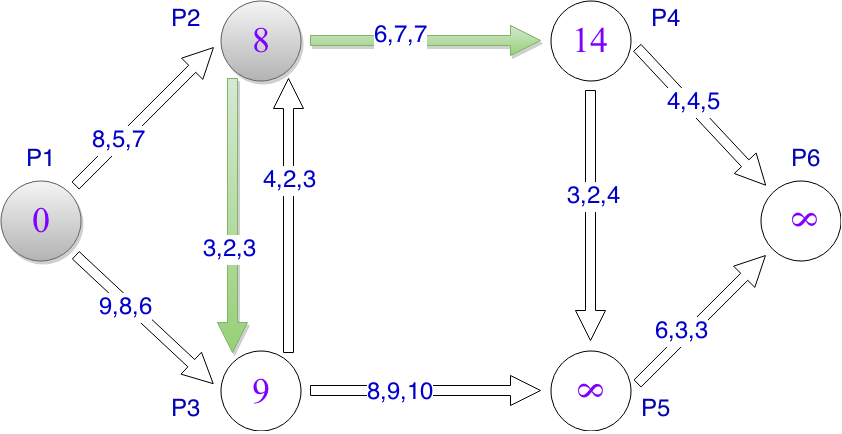
\includegraphics[width=.50\textwidth]{figuras/leo4.png}
\caption{Processo de determinação de caminho mínimo - Parte 3}
\label{fig:leo4}
\end{figure}
\FloatBarrier

\begin{table}[htbp]
  \centering
  \begin{tabular}{l l l l}
  \toprule
  Vértice & PERM & Distância & Predecessor\\
  \midrule
  P1 & Sim & 0 & - \\
  P2 & Sim & 8 & P1 \\
  P3 & Não & 9 & P1 \\
  P4 & Não & 14 & P2 \\
  P5 & Não & $\infty$ & - \\
  P6 & Não & $\infty$ & - \\
  \bottomrule
  \end{tabular}
\caption{Processo de determinação de caminho mínimo - Parte 3}
 \label{tab:leotab3}
\end{table}
\FloatBarrier

\begin{figure}[htbp]
\centering
 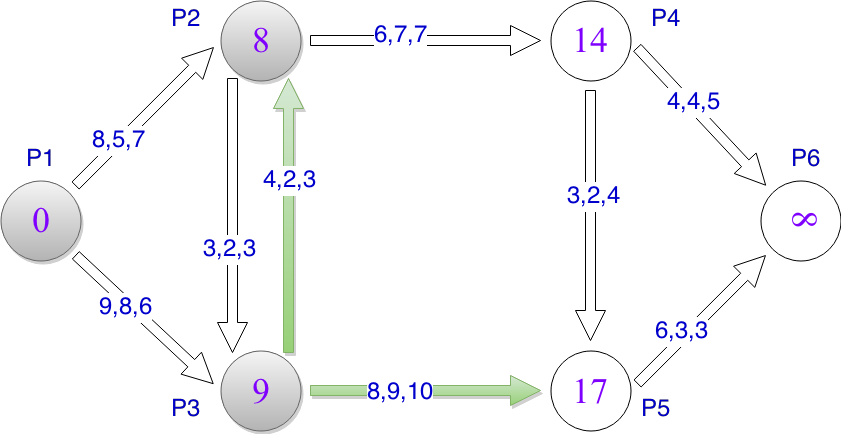
\includegraphics[width=.50\textwidth]{figuras/leo5.png}
\caption{Processo de determinação de caminho mínimo - Parte 4}
\label{fig:leo5}
\end{figure}

\begin{table}[htbp]
  \centering
  \begin{tabular}{l l l l}
  \toprule
  Vértice & PERM & Distância & Predecessor\\
  \midrule
  P1 & Sim & 0 & - \\
  P2 & Sim & 8 & P1 \\
  P3 & Sim & 9 & P1 \\
  P4 & Não & 14 & P2 \\
  P5 & Não & 17 & P3 \\
  P6 & Não & $\infty$ & - \\
  \bottomrule
  \end{tabular}
\caption{Processo de determinação de caminho mínimo - Parte 4}
 \label{tab:leotab4}
\end{table}
\FloatBarrier

Ao selecionar o vértice P4, não pertencente a PERM, o intervalo de previsão é ultrapassado
de 10 minutos. Logo, é utilizada a segunda posição do vetor de custos $t + 2$. O custo do trajeto até
o vértice P5 pelo P4 é menor do que o custo atual por P3, logo atualiza-se seu peso e predecessor
para 16 e P4 respectivamente.
\FloatBarrier
\begin{figure}[htbp]
\centering
 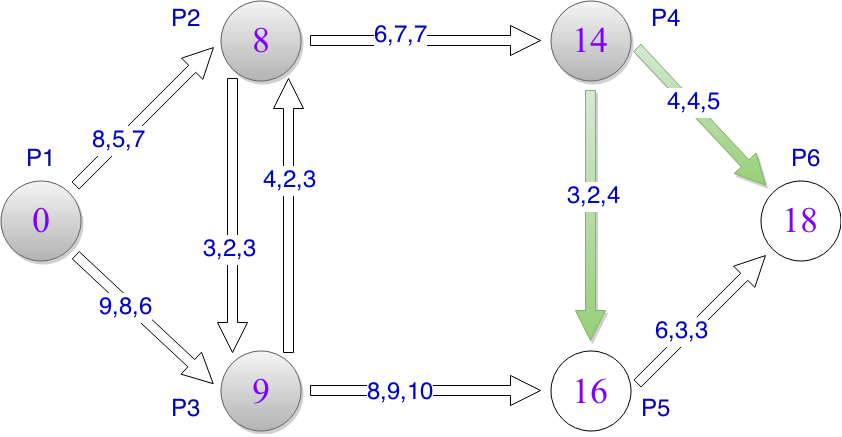
\includegraphics[width=.50\textwidth]{figuras/leo6.png}
\caption{Processo de determinação de caminho mínimo - Parte 5}
\label{fig:leo6}
\end{figure}

\begin{table}[htbp]
  \centering
  \begin{tabular}{l l l l}
  \toprule
  Vértice & PERM & Distância & Predecessor\\
  \midrule
  P1 & Sim & 0 & - \\
  P2 & Sim & 8 & P1 \\
  P3 & Sim & 9 & P1 \\
  P4 & Sim & 14 & P2 \\
  P5 & Não & 16 & P4 \\
  P6 & Não & 18 & P4 \\
  \bottomrule
  \end{tabular}
\caption{Processo de determinação de caminho mínimo - Parte 5}
 \label{tab:leotab5}
\end{table}

P5 é adicionado a PERM e seu único vértice adjacente é P6. Logo temos:
\FloatBarrier
\begin{figure}[htbp]
\centering
 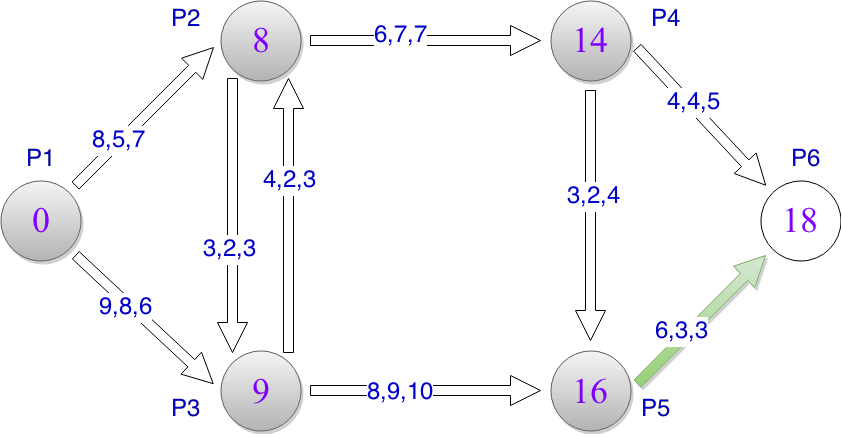
\includegraphics[width=.50\textwidth]{figuras/leo7.png}
\caption{Processo de determinação de caminho mínimo - Parte 6}
\label{fig:leo7}
\end{figure}

\begin{table}[htbp]
  \centering
  \begin{tabular}{l l l l}
  \toprule
  Vértice & PERM & Distância & Predecessor\\
  \midrule
  P1 & Sim & 0 & - \\
  P2 & Sim & 8 & P1 \\
  P3 & Sim & 9 & P1 \\
  P4 & Sim & 14 & P2 \\
  P5 & Sim & 16 & P4 \\
  P6 & Sim & 18 & P4 \\
  \bottomrule
  \end{tabular}
\caption{Processo de determinação de caminho mínimo - Parte 6}
 \label{tab:leotab5}
\end{table}
\FloatBarrier

E finalmente temos a figura \ref{fig:leo8}, pois P6 não possui vértice adjacente. Logo, o 
tempo para percorrer o caminho mínimo passando por P1, P2, P4 e P6 é 18 minutos.

\begin{figure}[htbp]
\centering
 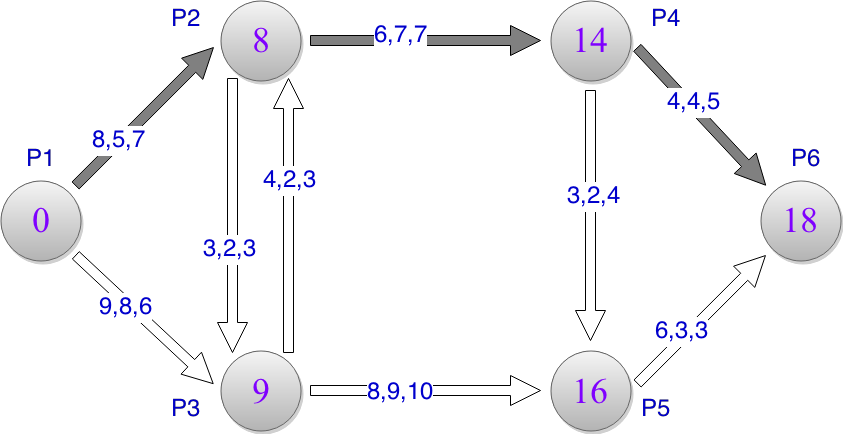
\includegraphics[width=.50\textwidth]{figuras/leo8.png}
\caption{Processo de determinação de caminho mínimo - Parte 7}
\label{fig:leo8}
\end{figure}
\FloatBarrier

A presente pesquisa resolve o mesmo problema utilizando o Algoritmo de Dijkstra com Radix Heap para Grafos Dinâmicos.
Foram implementados dois algoritmos nesse contexto: o primeiro segue a mesma abordagem do Dijkstra Modificado com Radix Heap
de \cite{leonard}, em relação a mudança do tempo de previsão ao exceder 10 minutos, chamado Algoritmo com Permissão Adiante;
e o segundo altera o intervalo de previsão quando o valor do custo do vértice acrescido do valor do custo da aresta adjacente 
for superior a 10, chamado Algoritmo sem Permissão Adiante.
Os dois usados em conjunto indicam um intervalo de limite inferior e superior para determinação do caminho mínimo.

Os dois algoritmos utilizam um vetor de custos composto pelo tempo médio das passagens dos veículos, em intervalos
de 10 minutos ao longo do dia, numa determinada ligação ou aresta. Por exemplo, entre 12 horas e 12 horas e 10 minutos um
veículo demora em média 2 minutos para percorrer a aresta, entre 12 horas e 10 minutos e 12h e 20 minutos ele demora 3 minutos
para percorrer a mesma aresta, e assim por diante. Os dados do vetor de custo são armazenados em um arquivo no formato JSON
como mostra a figura \ref{fig:tabelajson}. Cada aresta possui um vetor de tamanho 24 para representar as horas, e cada elemento
do vetor possui um vetor de tamanho 6 para representar os intervalos de 10 minutos ao longo de 1 hora.

\lstinputlisting[language=Java]{figuras/tabela.json}
\begin{figure}[htbp]
  \caption{Estrutura JSON usada pelo vetor de custos}
  \label{fig:tabelajson}
\end{figure}
\FloatBarrier

A mudança de intervalo de previsão do segundo algoritmo segue o seguinte exemplo: se o tempo parcial até um determinado 
ponto somado ao custo de travessia da aresta adjacente for de 8 minutos, então é utilizado para o próximo cálculo o tempo
de previsão no intervalo $t + 1$, mas se a soma for de 13 minutos, logo o período de previsão é ultrapassado, e com isso
utiliza-se $t + 2$ para o cálculo do próximo trajeto. Se a soma estiver entre 20 e 30 minutos utiliza-se o intervalo
$t + 3$, entre 30 e 40 minutos $t + 4$, e assim por diante.
O Algoritmo sem Permissão Adiante é representado pelo algoritmo \ref{codeRadix}, e o algoritmo \ref{sempermissaoadiante}
apresenta o pseudocódigo dessa abordagem, onde mostra a modificação do método na linha \ref{trechoradix} do
algoritmo \ref{codeRadix}.

\begin{algorithm}[h!]
\caption{Sem Permissão Adiante}
  \Inicio{
    custoAresta $\leftarrow$ horário até o momento\;
    \Se{custoAresta + custoVerticeSelecionado > janelaTemporalAtual}{
      custoAresta $\leftarrow$ tempo de previsão do próximo intervalo\;
    }
    \Se{custoAresta + custoVerticeSelecionado < custoVerticeDestino}{
      custoVerticeDestino $\leftarrow$ custoAresta + custoVerticeSelecionado\;
      predecessor verticeDestino $\leftarrow$ verticeSelecionado\;
    }
  }
\label{sempermissaoadiante}
\end{algorithm}
\FloatBarrier

A seguir, é apresentado o funcionamento do algoritmo utilizando o mesmo grafo da figura \ref{fig:leo1}
e o mesmo ponto de origem. Para determinar o caminho mínimo, cada vértice armazena o identificador do vértice anterior.
O algoritmo utiliza \textit{buckets} para armazenar os vértices de acordo com seus rótulos.
Inicialmente, os rótulos de todos os vértices recebem um custo de valor tendendo ao infinito exceto P1,
que possui custo 0, da mesma forma que a figura \ref{fig:leo2}. A figura \ref{fig:buckets} exibe a disposição dos vértices em seus
respectivos \textit{buckets}.

\begin{figure}[htbp]
\centering
 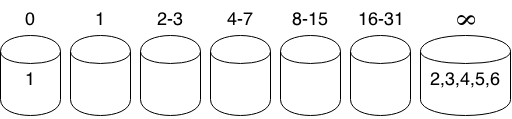
\includegraphics[width=.50\textwidth]{figuras/buckets.png}
\caption{Disposição dos vértices nos buckets}
\label{fig:buckets}
\end{figure}
\FloatBarrier

Após consultar os vértices adjacentes a P1, que são P2 e P3, o pseudocódigo \ref{sempermissaoadiante}
é executado e o mesmo resultado da figura \ref{fig:leo3} é encontrado. Em seguida, os \textit{buckets} são atualizados
como mostra a figura \ref{fig:buckets1}.

\begin{figure}[htbp]
\centering
 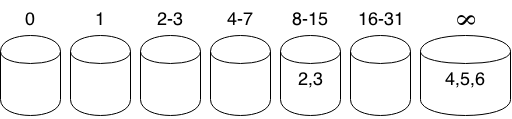
\includegraphics[width=.50\textwidth]{figuras/buckets1.png}
\caption{Disposição dos vértices nos buckets - Parte 1}
\label{fig:buckets1}
\end{figure}
\FloatBarrier

Como o menor \textit{bucket} não tem largura igual a 1 e possui mais de 1 elemento, o intervalo dos \textit{buckets}
é atualizado:

\begin{figure}[htbp]
\centering
 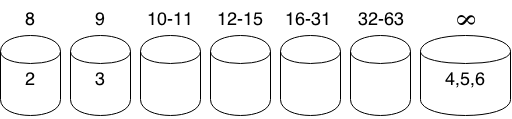
\includegraphics[width=.50\textwidth]{figuras/buckets2.png}
\caption{Disposição dos vértices nos buckets - Parte 2}
\label{fig:buckets2}
\end{figure}
\FloatBarrier

O vértice P2 é selecionado do menor \textit{bucket} e em seguida consulta-se seus vértices adjacentes, que são P3 e P4.
O intervalo de previsão é ultrapassado ao somar o rótulo de P2 com o custo da aresta, que segue até P3, no intervalo $t + 1$. Logo, 
é utilizado a próxima posição do vetor de custos, que é $t + 2$. As figuras \ref{fig:limitesup1} e \ref{fig:buckets3} exibem o resultado.

\begin{figure}[htbp]
\centering
 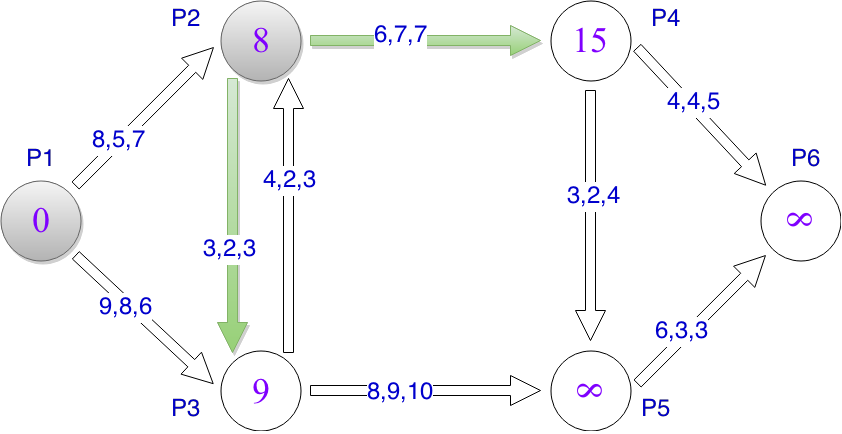
\includegraphics[width=.50\textwidth]{figuras/limitesup1.png}
\caption{Radix Heap - Parte 1}
\label{fig:limitesup1}
\end{figure}

\begin{figure}[htbp]
\centering
 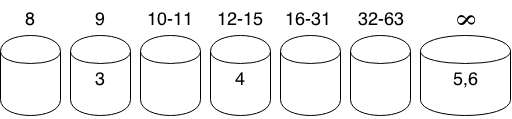
\includegraphics[width=.50\textwidth]{figuras/buckets3.png}
\caption{Disposição dos vértices nos buckets - Parte 3}
\label{fig:buckets3}
\end{figure}
\FloatBarrier

Em seguida, são exibidos os próximos passos até chegar no resultado final.
\begin{figure}[htbp]
\centering
 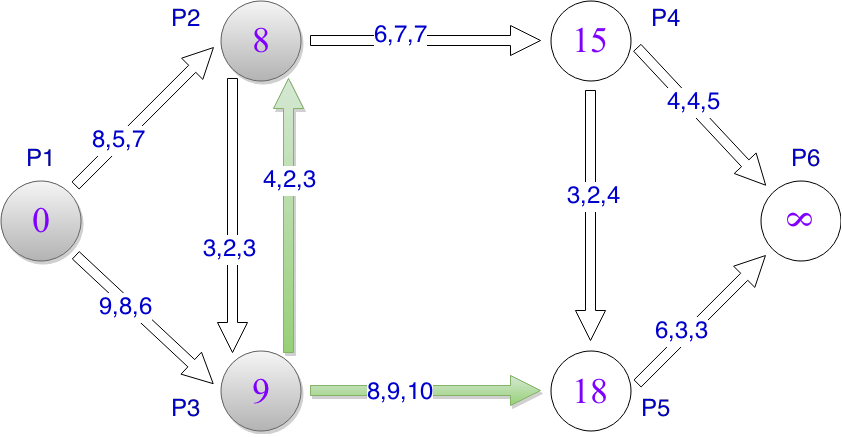
\includegraphics[width=.50\textwidth]{figuras/limitesup2.png}
\caption{Radix Heap - Parte 2}
\label{fig:limitesup2}
\end{figure}

\begin{figure}[htbp]
\centering
 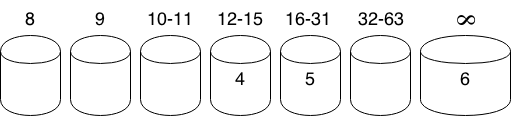
\includegraphics[width=.50\textwidth]{figuras/buckets4.png}
\caption{Disposição dos vértices nos buckets - Parte 4}
\label{fig:buckets4}
\end{figure}
\FloatBarrier

\begin{figure}[htbp]
\centering
 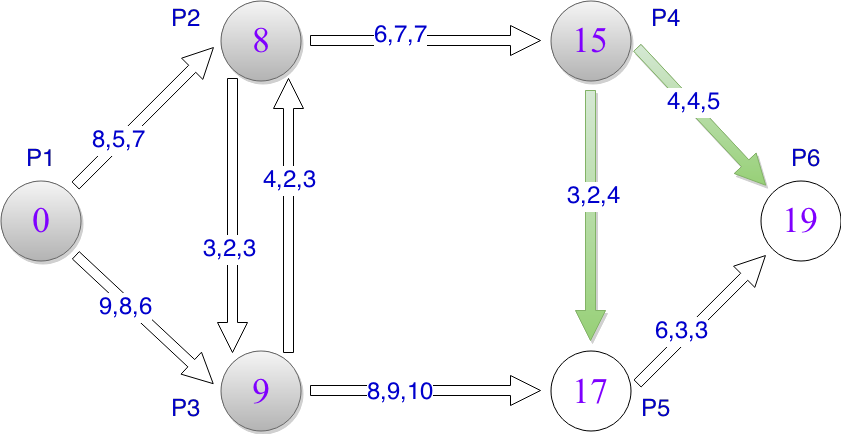
\includegraphics[width=.50\textwidth]{figuras/limitesup3.png}
\caption{Radix Heap - Parte 3}
\label{fig:limitesup3}
\end{figure}

\begin{figure}[htbp]
\centering
 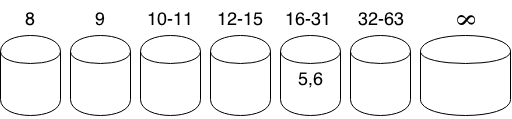
\includegraphics[width=.50\textwidth]{figuras/buckets5.png}
\caption{Disposição dos vértices nos buckets - Parte 5}
\label{fig:buckets5}
\end{figure}
\FloatBarrier

Novamente o intervalo dos ``buckets'' é atualizado e P5 é selecionado.
\begin{figure}[htbp]
\centering
 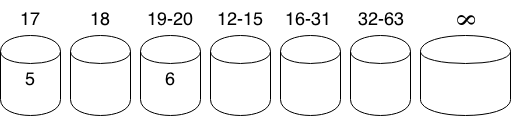
\includegraphics[width=.50\textwidth]{figuras/buckets6.png}
\caption{Disposição dos vértices nos buckets - Parte 6}
\label{fig:buckets6}
\end{figure}
\FloatBarrier
\begin{figure}[htbp]
\centering
 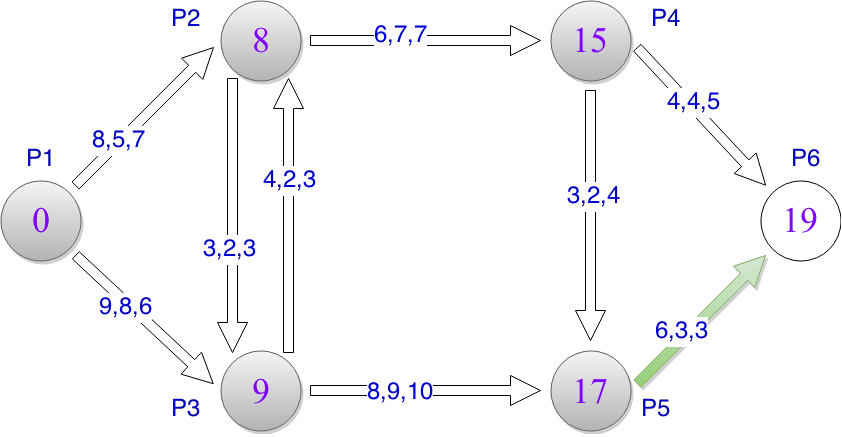
\includegraphics[width=.50\textwidth]{figuras/limitesup4.png}
\caption{Radix Heap - Parte 4}
\label{fig:limitesup4}
\end{figure}
\FloatBarrier
\begin{figure}[htbp]
\centering
 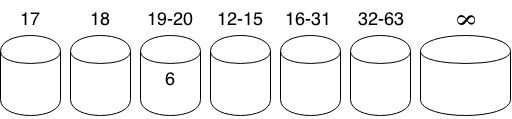
\includegraphics[width=.50\textwidth]{figuras/buckets7.png}
\caption{Disposição dos vértices nos buckets - Parte 7}
\label{fig:buckets7}
\end{figure}
\FloatBarrier

Finalmente, P6 é selecionado, mas como não possui vértices adjacentes, o caminho mínimo é definido passando
pelos vértices P1, P2, P4 e P6 com tempo de percurso de 19 minutos, como mostra a figura \ref{fig:limitesup5}.

\begin{figure}[htbp]
\centering
 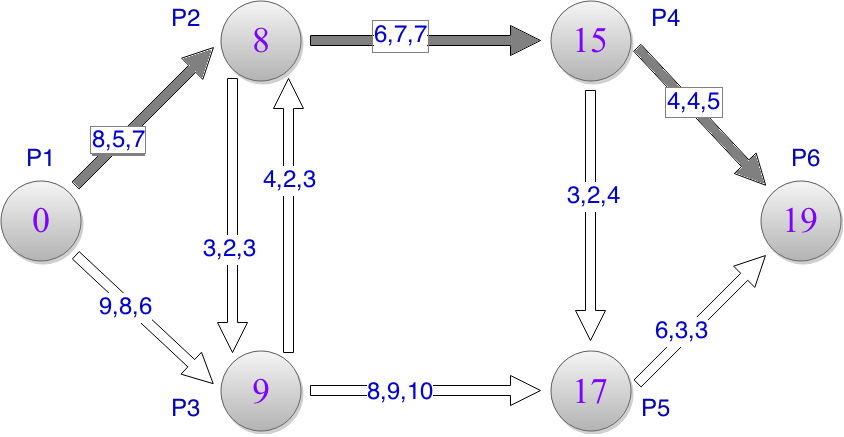
\includegraphics[width=.50\textwidth]{figuras/limitesup5.png}
\caption{Radix Heap - Parte 5}
\label{fig:limitesup5}
\end{figure}
\FloatBarrier

Tomando-se o grafo da figura \ref{fig:leo8} e o grafo da figura \ref{fig:limitesup5}, vimos que os percursos
foram os mesmos $P1 \rightarrow P2 \rightarrow P4 \rightarrow P6$ porém os custos (tempos) foram distintos.
No primeiro algoritmo, obtivemos o tempo mínimo de percurso de 18 minutos, enquanto no segundo obtivemos 19 minutos.
Nota-se aqui que a visão adiante ou robusta afeta diretamente o cálculo do caminho mínimo (tempo) no grafo dinâmico,
apesar de não ter afetado a discrição do percurso.
Porém deve-se tomar cuidado, pois os percursos para cada método podem ser distintos.

% O exemplo da figura \ref{fig:intervalo} exibe a resolução dos caminhos mínimos de dois grafos de vetor de custo distintos,
% usando os dois algoritmos implementados nesta pesquisa. 
% \begin{figure}[htbp]
% \centering
%  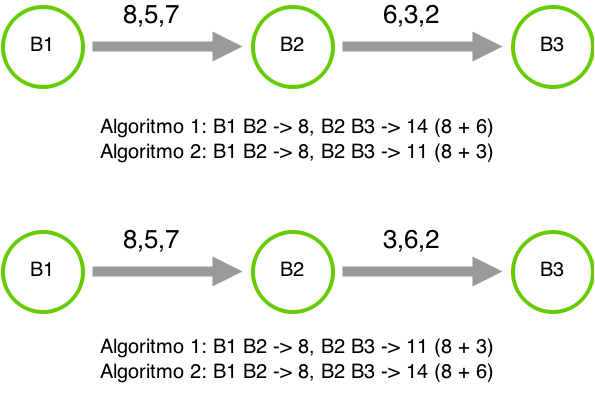
\includegraphics[width=.60\textwidth]{figuras/intervalo.png}
% \caption{Grafo exemplo para indicar o Intervalo de Previsão}
% \label{fig:intervalo}
% \end{figure}
% \FloatBarrier

\subsubsection{Topologia Dinâmica e Atributos Estáticos}
Esse algoritmo não foi implementado e segue a estrutura apresentada na seção \ref{subsec:topdinatribest},
onde vértices e arestas podem mudar ao longo do tempo e seus atributos são constantes. A 
figura \ref{fig:pathtopdyn} apresenta essa estrutura:

\begin{figure}[htbp]
\centering
 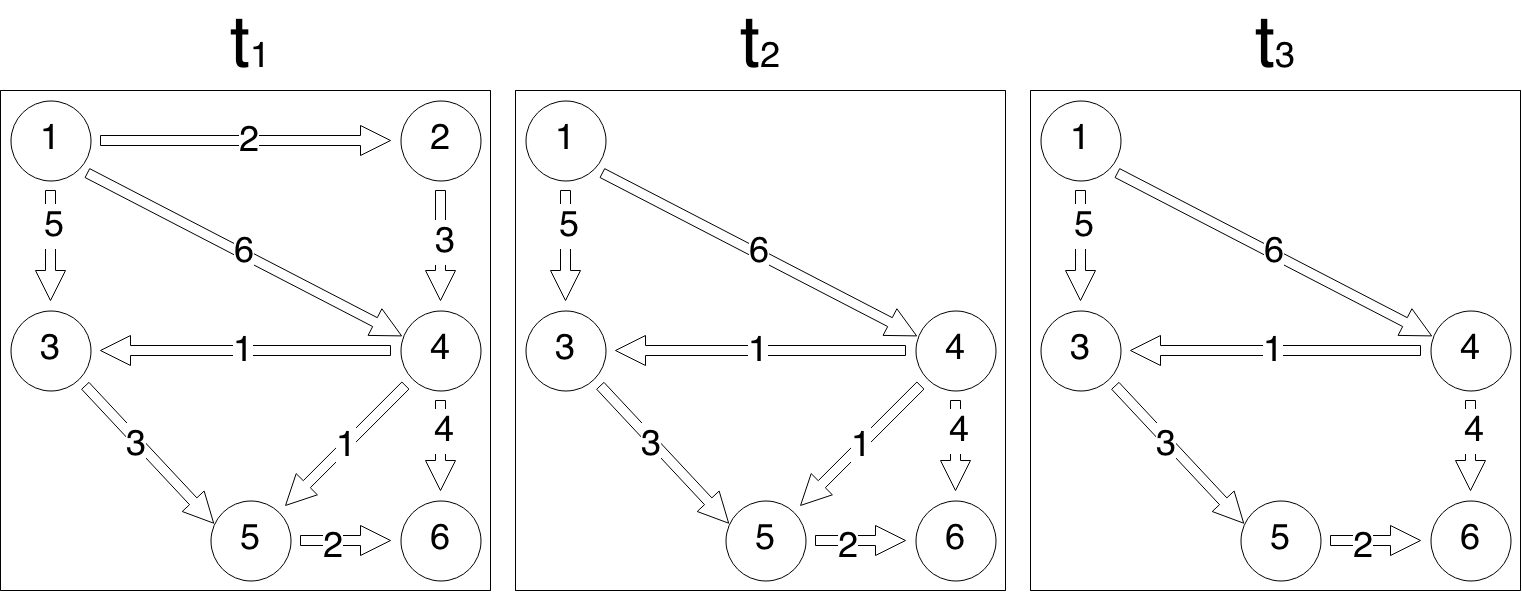
\includegraphics[width=.80\textwidth]{figuras/pathtopdyn.png}
\caption{Caminho Mínimo - Topologia Dinâmica e Atributos Estáticos}
\label{fig:pathtopdyn}
\end{figure}
\FloatBarrier
O exemplo utiliza pontos representados através do grafo G(N=\{P1, P2, P3, P4, P5, P6\}, A), onde o 
ponto de partida é P1 e o destino o ponto P6. No instante $t_1$ é possível observar vários caminhos
até chegar ao objetivo. Já no instante $t_2$ o vértice P2 foi removido, e em $t_3$ a aresta que começa em
P4 e vai até P5 é removida, e com isso reduzindo as possibilidades de chegar a P6. Diante disso,
se faz necessário conhecer o tempo inicial e final de cada vértice e aresta para chegar a P6.

\subsubsection{Topologia Dinâmica e Atributos Dinâmicos}
Essa seção resolve o problema apresentado na seção \ref{subsec:limitesuperior} utilizando o Algoritmo de
Dijkstra com Radix Heap seguindo a estrutura da seção \ref{subsec:topdinatridin}.

Ao executar o exemplo da figura \ref{fig:leo1}, com o mesmo vetor de custo e ponto de origem, tem-se
os vértices adjacentes P2 e P3. Ao atualizar o rótulo dos vértices adjacentes, é necessário executar o mesmo
pseudocódigo \ref{sempermissaoadiante}. Além disso, é levado em consideração o tempo
inicial e final dos vértices e arestas para determinar o caminho mínimo. Para isso,
verifica-se as seguintes questões:
\begin{itemize}
\item Se a aresta já existe, ou seja, se o tempo inicial dela é menor que o horário de referência;
\item Se a aresta existirá durante o tempo de travessia, que correspondente ao seu custo no intervalo de previsão;
\item Se os vértices origem e destino existirão durante a travessia.
\end{itemize}
\FloatBarrier

O algoritmo, fica, pois do seguinte modo:

\begin{algorithm}[h!]
\caption{Radix Heap - Topologia Dinâmica e Atributos Dinâmicos}
  \Inicio{
    \Para{isValidPath(elemento, horarioDestino, horarioOrigem)}{
      ini $\leftarrow$ data inicial do elemento\;
      \Se {ini > horarioOrigem}{
        O elemento ainda não existe \Return falso\;
      }
      \Se {data final do elemento for diferente de nulo}{
        fim $\leftarrow$ data final do elemento\;
        Return (fim > horarioDestino $\&\&$ horarioDestino > ini)\;
      }
      Return horarioDestino > ini\;
    }

    horarioOrigem $\leftarrow$ horário de referência\;
    horarioDestino $\leftarrow$ horário de referência\;
    isValidLigacao $\leftarrow$ isValidPath(ligacao, horarioDestino, horarioOrigem)\;
    isValidVerticeOrigem $\leftarrow$ isValidPath(verticeOrigem, horarioDestino)\;
    isValidVerticeDestino $\leftarrow$ isValidPath(verticeDestino, horarioDestino, horarioOrigem)\;

    \Se {!isValidLigacao $\|\|$ !isValidVerticeOrigem $\|\|$ !isValidVerticeDestino}{
      custoVerticeDestino $\leftarrow$ custoOriginal\;
      predecessor[v] $\leftarrow$ predecessor anterior\;
    }
  }
\label{algtudodinamico}
\end{algorithm}
\FloatBarrier

Para ilustrar o método proposto para este tipo de rede, consideramos o seguinte grafo da figura \ref{fig:datatime}, que
exibe o tempo de existência de cada elemento do grafo.

\lstinputlisting[language=Java]{figuras/datatime.json}
\begin{figure}[htbp]
  \caption{Estrutura JSON do tempo de existência dos vértices e arestas}
  \label{fig:datatime}
\end{figure}
\FloatBarrier

A seguir, é exibido o grafo dinâmico na figura \ref{fig:datatime} para acompanhar o exemplo.

\begin{figure}[htbp]
\centering
 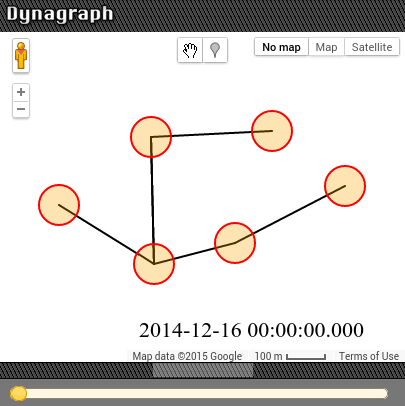
\includegraphics[width=.45\textwidth]{figuras/explicacaoDyn1.png}
 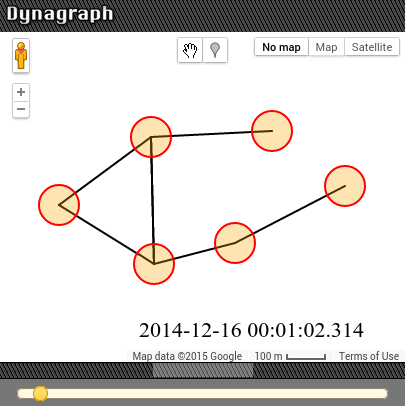
\includegraphics[width=.45\textwidth]{figuras/explicacaoDyn2.png}
 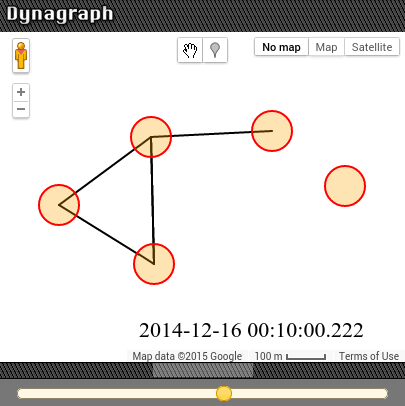
\includegraphics[width=.45\textwidth]{figuras/explicacaoDyn3.png}
 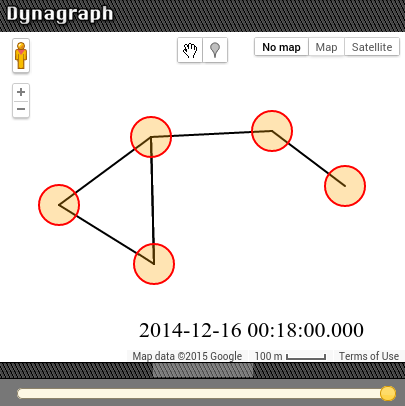
\includegraphics[width=.45\textwidth]{figuras/explicacaoDyn4.png}
\caption{Dynagraph - Captura de tela}
\label{fig:explicacaodyn}
\end{figure}
\FloatBarrier

A figura \ref{fig:dyndyn1} exibe o início da solução do caminho sobre o grafo dinâmico.
Tomando os vértices adjacentes a P1, observa-se o grafo da figura \ref{fig:dyndyn1}, onde as arestas
que ligam P1 a P2 e P4 a P5 ainda não existem.

\begin{figure}[htbp]
\centering
 \includegraphics[width=.55\textwidth]{figuras/dyndyn1.png}
\caption{Radix Heap Dinâmico - Parte 1}
\label{fig:dyndyn1}
\end{figure}
\FloatBarrier

A seguir, é apresentada a sequência de instantes utilizando o Dynagraph após resolução do algoritmo.

\begin{figure}[htbp]
\centering
 \includegraphics[width=.42\textwidth]{figuras/dyndyn2.png}
 \includegraphics[width=.42\textwidth]{figuras/dyndyn3.png}
\caption{Radix Heap Dinâmico - Parte 2 e 3}
\label{fig:dyndyn2}
\end{figure}

\begin{figure}[htbp]
\centering
 \includegraphics[width=.42\textwidth]{figuras/dyndyn4.png}
 \includegraphics[width=.42\textwidth]{figuras/dyndyn5.png}
\caption{Radix Heap Dinâmico - Parte 4 e 5}
\label{fig:dyndyn3}
\end{figure}

\begin{figure}[htbp]
\centering
 \includegraphics[width=.42\textwidth]{figuras/dyndyn6.png}
 \includegraphics[width=.42\textwidth]{figuras/dyndyn7.png}
\caption{Radix Heap Dinâmico - Parte 6 e 7}
\label{fig:dyndyn4}
\end{figure}


	\chapter{Validação}

Para validação dos algoritmos foram gerados alguns grafos hipotéticos com cenários distintos.
Alguns deles utilizam o mesmo vetor de custo, como dito na seção \ref{sec:pathdyn}, que representam
o tempo médio das passagens dos veículos por uma aresta ao longo do dia, em intervalos padrões (10 minutos para nosso caso).

\section{Ferramenta de cálculo do caminho mínimo}
Para determinar o caminho mínimo entre dois vértices conhecidos em grafos dinâmicos, foi construída uma ferramenta (\textit{software})
extendida do Dynagraph, que calcula o caminho mínimo. Para isso, em um grafo dinâmico segue a sequência:
\begin{itemize}
\item Ler a estrutura de dados JSON;
\item Exibir o grafo com todos os vértices e arestas;
\item Selecionar um dos algoritmos para cálculo e exibição do caminho mínimo;
\item Baixar o arquivo JSON ou ir para a aplicação Dynagraph, que contém os mesmos dados do grafo mais as arestas do caminho mínimo;
\end{itemize}

As figuras \ref{fig:shortestpath}, \ref{fig:upperlimit} e \ref{fig:downlimit} mostram captura de telas
da ferramenta exibindo exemplos de caminho mínimo dos algoritmos e os seus dados em um determinado tipo de rede:

\begin{figure}[htbp]
\centering
 \includegraphics[width=.90\textwidth]{figuras/validacao/shortestpath.png}
\caption{Simulador de Caminho Mínimo - Topologia Dinâmica e Atributos Dinâmicos}
\label{fig:shortestpath}
\end{figure}
\FloatBarrier

\begin{figure}[htbp]
\centering
 \includegraphics[width=.90\textwidth]{figuras/validacao/upperlimit.png}
\caption{Simulador de Caminho Mínimo - Topologia Estática e Atributos Dinâmicos: sem permissão adiante}
\label{fig:upperlimit}
\end{figure}
\FloatBarrier

\begin{figure}[htbp]
\centering
 \includegraphics[width=.90\textwidth]{figuras/validacao/downlimit.png}
\caption{Simulador de Caminho Mínimo - Topologia Estática e Atributos Dinâmicos: com permissão adiante}
\label{fig:downlimit}
\end{figure}
\FloatBarrier

\lstinputlisting[language=Java]{figuras/dataex1.json}
\begin{figure}[htbp]
  \caption{Estrutura JSON - Exemplo 1}
  \label{fig:jsondyn}
\end{figure}
\FloatBarrier

A seguir, são apresentados os grafos gerados pela ferramenta com seus respectivos dados,
e a exibição do caminho mínimo no Dynagraph. As figuras seguem a ordem da esquerda para a direita e
de cima para baixo.

\begin{figure}[htbp]
\centering
 \includegraphics[width=.70\textwidth]{figuras/validacao/ex1.png}
\caption{Simulador de Caminho Mínimo - Exemplo 1}
\label{fig:ex1}
\end{figure}
\FloatBarrier

\begin{figure}[htbp]
\centering
 \includegraphics[width=.25\textwidth]{figuras/validacao/dyn1a.png}
 \includegraphics[width=.25\textwidth]{figuras/validacao/dyn1b.png}
 \includegraphics[width=.25\textwidth]{figuras/validacao/dyn1c.png}
 \includegraphics[width=.25\textwidth]{figuras/validacao/dyn1d.png}
\caption{Caminho Mínimo no Dynagraph - Exemplo 1}
\label{fig:dyn1}
\end{figure}
\FloatBarrier

\lstinputlisting[language=Java]{figuras/validacao/dyn1.json}
\begin{figure}[htbp]
  \caption{Simulador de Caminho Mínimo: Estrutura JSON - Exemplo 1}
  \label{fig:jsondyn1}
\end{figure}
\FloatBarrier


\begin{figure}[htbp]
\centering
 \includegraphics[width=.70\textwidth]{figuras/validacao/ex2.png}
\caption{Simulador de Caminho Mínimo - Exemplo 2}
\label{fig:ex2}
\end{figure}
\FloatBarrier

\begin{figure}[htbp]
\centering
 \includegraphics[width=.35\textwidth]{figuras/validacao/dyn2a.png}
 \includegraphics[width=.35\textwidth]{figuras/validacao/dyn2b.png}
 \includegraphics[width=.35\textwidth]{figuras/validacao/dyn2c.png}
 \includegraphics[width=.35\textwidth]{figuras/validacao/dyn2d.png}
\caption{Caminho Mínimo no Dynagraph - Exemplo 2}
\label{fig:dyn2}
\end{figure}
\FloatBarrier

\lstinputlisting[language=Java]{figuras/validacao/dyn2.json}
\begin{figure}[htbp]
  \caption{Simulador de Caminho Mínimo: Estrutura JSON - Exemplo 2}
  \label{fig:jsondyn2}
\end{figure}
\FloatBarrier

A seguir, o mesmo exemplo do grafo anterior, mas com o horário de início do percurso diferente.
Percebe-se que a hora é ultrapassada, pois o percurso inicia às 23 horas e 50 minutos.
% Considerando o grafo G(N=\{P1, P2, P3, P4, P5, P6\}, A), o caminho determinado parte de P1, passa por P4 e chega em P6.

\begin{figure}[htbp]
\centering
 \includegraphics[width=.70\textwidth]{figuras/validacao/ex3.png}
\caption{Simulador de Caminho Mínimo - Exemplo 3}
\label{fig:ex3}
\end{figure}
\FloatBarrier

\begin{figure}[htbp]
\centering
 \includegraphics[width=.35\textwidth]{figuras/validacao/dyn3a.png}
 \includegraphics[width=.35\textwidth]{figuras/validacao/dyn3b.png}
 \includegraphics[width=.35\textwidth]{figuras/validacao/dyn3c.png}
\caption{Caminho Mínimo no Dynagraph - Exemplo 3}
\label{fig:dyn3}
\end{figure}
\FloatBarrier

\lstinputlisting[language=Java]{figuras/validacao/dyn3.json}
\begin{figure}[htbp]
  \caption{Simulador de Caminho Mínimo: Estrutura JSON - Exemplo 3}
  \label{fig:jsondyn3}
\end{figure}
\FloatBarrier

Logo abaixo, um exemplo usando o mesmo vetor de custo do exemplo 3.

\begin{figure}[htbp]
\centering
 \includegraphics[width=.70\textwidth]{figuras/validacao/ex4.png}
\caption{Simulador de Caminho Mínimo - Exemplo 4}
\label{fig:ex4}
\end{figure}
\FloatBarrier

\begin{figure}[htbp]
\centering
 \includegraphics[width=.35\textwidth]{figuras/validacao/dyn4a.png}
 \includegraphics[width=.35\textwidth]{figuras/validacao/dyn4b.png}
 \includegraphics[width=.35\textwidth]{figuras/validacao/dyn4c.png}
 \includegraphics[width=.35\textwidth]{figuras/validacao/dyn4d.png}
 \includegraphics[width=.35\textwidth]{figuras/validacao/dyn4e.png}
 \includegraphics[width=.35\textwidth]{figuras/validacao/dyn4f.png}
 \includegraphics[width=.35\textwidth]{figuras/validacao/dyn4g.png}
 \includegraphics[width=.35\textwidth]{figuras/validacao/dyn4h.png}
\caption{Caminho Mínimo no Dynagraph - Exemplo 4}
\label{fig:dyn4}
\end{figure}
\FloatBarrier

\lstinputlisting[language=Java]{figuras/validacao/dyn4.json}
\begin{figure}[htbp]
  \caption{Simulador de Caminho Mínimo: Estrutura JSON - Exemplo 4}
  \label{fig:jsondyn4}
\end{figure}
\FloatBarrier

\begin{figure}[htbp]
\centering
 \includegraphics[width=.70\textwidth]{figuras/validacao/ex5.png}
\caption{Simulador de Caminho Mínimo - Exemplo 5}
\label{fig:ex5}
\end{figure}
\FloatBarrier

\begin{figure}[htbp]
\centering
 \includegraphics[width=.35\textwidth]{figuras/validacao/dyn5a.png}
 \includegraphics[width=.35\textwidth]{figuras/validacao/dyn5b.png}
 \includegraphics[width=.35\textwidth]{figuras/validacao/dyn5c.png}
 \includegraphics[width=.35\textwidth]{figuras/validacao/dyn5d.png}
 \includegraphics[width=.35\textwidth]{figuras/validacao/dyn5e.png}
 \includegraphics[width=.35\textwidth]{figuras/validacao/dyn5f.png}
\caption{Caminho Mínimo no Dynagraph - Exemplo 5}
\label{fig:dyn5}
\end{figure}
\FloatBarrier

\lstinputlisting[language=Java]{figuras/validacao/dyn5.json}
\begin{figure}[htbp]
  \caption{Simulador de Caminho Mínimo: Estrutura JSON - Exemplo 5}
  \label{fig:jsondyn5}
\end{figure}
\FloatBarrier
	\chapter{Conclusões e Trabalhos Futuros}

O presente trabalho utilizou algoritmos de caminho mínimo em grafos dinâmicos
para determinação de percusos com tempo mínimo em grafos hipotéticos.
A aplicação destes algoritmos resultou na formulação de um modelo computacional em grafos
de topologia dinâmica e atributos dinâmicos. Também foi construída uma ferramenta (\textit{software})
extendida do Dynagraph, que calcula e exibe o caminho mínimo entre dois vértices conhecidos.

Inicialmente foram apresentados os algoritmos de topologia estática e atributos dinâmicos com
limite inferior e superior. Em seguida, esses mesmos algoritmos foram utilizados no algoritmo
de topologia dinâmica e atributos dinâmicos.

Pode-se concluir que o algoritmo utilizado em grafos de topologia dinâmica e atributos dinâmicos
é eficiente ao ponto de garantir a resolução do problema dentro dos objetivos propostos, pois ele
garante um intervalo de previsão para travessia de cada aresta e intervalo para o caminho mínimo.
Mesmo sabendo que o modelo não é o mais eficiente, pois o mesmo é implementado usando o
algoritmo de Dijkstra com Radix Heap, e poderia usar a estrutura de dados Fibonacci heap com a
implementação do radix heap, e com isso reduzir ainda mais a complexidade.

Esta pesquisa também contribuiu com a integração da ferramenta implementada com a ferramenta Dynagraph.
Essa integração permite através do Dynagraph solicitar o caminho mínimo do grafo em análise. Para isso, ele faz 
uma chamada ao \textit{software} deselvolvido. Este, por sua vez, analisa o grafo enviado, calcula o caminho mínimo
e envia para o Dynagraph o mesmo grafo acrescido das arestas do caminho mínimo gerado.

Para trabalho futuros, pretende-se provar que o algoritmo de caminho mínimo para grafos dinâmicos implementado garante que o
intervalo de previsão é mínimo. Também pretende-se otimizar o algoritmo para garantir o cálculo eficiente, pois a pesquisa
somente se concentrou na elaboração do modelo computacional.
Para trabalhos futuros na ferramenta, pretende-se resolver alguns detalhes para garantir o funcionamento da ferramenta.
A aplicação ainda limita-se ao selecionar um grafo em arquivo externo, pois o mesmo seleciona um grafo na implementação.
Pretende-se disponibilizar uma opção na ferramenta que indique o horário inicial de partida
do caminho mínimo. E por fim, aperfeiçoar o Editor de Características extendendo a edição para arestas e integrar ao Dynagraph.

	
	%Elementos pós-textuais	
	\bibliography{elementos-pos-textuais/referencias}
	%\imprimirglossario	
	%\imprimirapendices
		% Adicione aqui os apendices do seu trabalho
		%\apendice{Lorem Ipsum}
\label{ap:lorem-ipsum}

\lipsum[1]
		%\apendice{Modelo de Capa}
\label{ap:modelo-de-capa}

\lipsum[1]

		%\apendice{Termo de Fiel Depositário}
\label{ap:termo-de-fiel-depositario}

\noindent \textbf{Pesquisa:} ANÁLISE DA MORTALIDADE INFANTIL COM MALFORMAÇÕES CONGÊNITAS.

\noindent Pelo presente instrumento que atende às exigências legais, a Sra. Maria Consuelo Martins Saraiva, ``fiel depositário'' com o cargo de Secretária Municipal de Saúde de Iracema, após ter tomado conhecimento do protocolo de pesquisa intitulado: ANÁLISE DA MORTALIDADE INFANTIL COM MALFORMAÇÕES CONGÊNITAS. Analisando a repercussão desse estudo no contexto da saúde pública e epidemiologia, autoriza Karla Maria da Silva Lima, enfermeira, aluna do Curso de Mestrado Acadêmico em Enfermagem da Universidade Estadual do Ceará (UECE), sob orientação do Prof. Dr. José Maria de Castro, da UECE, ter acesso aos bancos de dados do Sistema de Informação sobre Nascidos Vivos e do Sistema de Informação sobre Mortalidade da Secretaria Municipal de Saúde de Iracema, objeto deste estudo, e que se encontram sob sua total responsabilidade. Fica claro que o Fiel Depositário pode a qualquer momento retirar sua AUTORIZAÇÃO e ciente de que todas as informações prestadas tornar-se-ão confidenciais e guardadas por força de sigilo profissional, assegurando que os dados obtidos da pesquisa serão somente utilizados para estudo.	
	%\imprimiranexos
		% Adicione aqui os anexos do seu trabalho
		%\anexo{Exemplo de Anexo}
\label{an:exemplo-de-anexo}

\lipsum[13]		
		%\anexo{Dinâmica das classes sociais}
\label{an:dinamica-das-classes-sociais}

\lipsum[14]
\index{AAA}
	%\imprimirindice

\end{document}